% Two-column paper style, max 10 pages
\documentclass[9pt,twocolumn]{article}
\usepackage[top=1.8cm,bottom=2cm,left=1.4cm,right=1.4cm,columnsep=0.45cm]{geometry}
\usepackage{graphicx}
\usepackage{amsmath,amssymb}
\usepackage{algorithm}
\usepackage{algpseudocode}
\usepackage[utf8]{inputenc}
\usepackage[T1]{fontenc}
\usepackage{booktabs}
\usepackage[hidelinks]{hyperref}
\usepackage{placeins}
\usepackage{float}
\usepackage[backend=bibtex]{biblatex}
\addbibresource{sample.bib}
\usepackage{titlesec}
\usepackage{microtype}
\usepackage{xcolor}
\usepackage{authblk}
\usepackage{stfloats}   % allow figure* at bottom of page
\usepackage{enumitem}

% Tighter section spacing
\titlespacing*{\section}{0pt}{6pt}{3pt}
\titlespacing*{\subsection}{0pt}{4pt}{2pt}
\titleformat{\section}{\normalsize\bfseries}{\thesection}{0.5em}{}
\titleformat{\subsection}{\small\bfseries}{\thesubsection}{0.5em}{}

\setlength{\parskip}{2pt}
\setlength{\parindent}{1em}
\setlength{\abovecaptionskip}{4pt}
\setlength{\belowcaptionskip}{0pt}
\setlength{\floatsep}{6pt}
\setlength{\textfloatsep}{6pt}

% Compact captions
\usepackage[font=small,labelfont=bf,skip=3pt]{caption}

\title{\large\textbf{\textit{Chaos Control and Schedule of Shuttle Buses}
\normalfont\normalsize\ [Nagatani, 2006]}}

\author[1]{Tran Quang Hung}
\author[1]{Le Gia Huy}
\author[1]{Nguyen Hoang Son Tung}
\affil[1]{\small School of Information and Communications Technology,
Hanoi University of Science and Technology\protect\newline
\textbf{Supervisor: PhD.\ Bui Quoc Trung}}
\date{}

\begin{document}

% ── HUST Cover Page ──────────────────────────────────────────────────────────
\begin{titlepage}
\begin{center}
\textsc{\large\textbf{HANOI UNIVERSITY OF SCIENCE AND TECHNOLOGY}}\\[0.5cm]
{\large\textbf{\uppercase{School of Information and Communications Technology}}\\[1cm]}

\includegraphics[scale=0.13]{logo-soict-hust-1.png}\\[1cm]
\textsc{\Large\textbf{Project Report}}\\[0.4cm]
\rule{\linewidth}{0.7mm}\\[0.4cm]
{\huge\bfseries\color{black!70!black} Chaos Control and Schedule of Shuttle Buses\\[0.4cm]}
\rule{\linewidth}{0.7mm}\\[1cm]

\color{black!80!black}{\large\textbf{\textit{Supervised by:}}}\\[0.4cm]
\begin{tabular}{l}
\large\textbf{PhD.\ Bui Quoc Trung}\\[1cm]
\end{tabular}

\color{black!80!black}{\large\textbf{\textit{Presented by:}}}\\[0.4cm]
\color{black}
\begin{tabular}{l@{\hspace{1.5cm}}r}
\large Tran Quang Hung & \large 20235502\\[0.4cm]
\large Nguyen Hoang Son Tung & \large 20225536\\[0.4cm]
\large Le Gia Huy & \large 20225498\\[0.4cm]
\end{tabular}

\vfill
{\large\color{black!80!black}{\textbf{Hanoi -- Vietnam}}\\[0.2cm]
\color{blue!90!black}\textbf{2026}}
\end{center}
\end{titlepage}
\setcounter{page}{1}

\twocolumn[{%
\maketitle
\vspace{-1em}
\begin{center}
\begin{minipage}{0.92\textwidth}
\small\textbf{Abstract.}
We reproduce all figures of Nagatani (2006)~\cite{nagatani}, which models $M$ shuttle buses as a discrete nonlinear map driven by passenger loading. An event-driven, min-heap simulator iterates $T_i(m+1)=T_i(m)+\Gamma H_i(m)+1/(1+S_i H_i(m))$ for arbitrary $M$ and per-bus speedup $S_i$. We confirm the paper's key results: the system undergoes period-adding bifurcations ($3\!\to\!5\!\to\!7\!\to\cdots$) rather than period-doubling as the loading parameter $\Gamma$ increases, with the onset delayed by higher speedup $S$; return maps exhibit deterministic piecewise-linear structure distinguishing chaos from noise; and the phase boundary $\Gamma^*(S)$ is found by bisection. We additionally show the model is robust to initial conditions and persists under additive noise up to 5\% of the mean headway. Extending to $M=3$ buses requires no new model: every qualitative insight carries over, with two new effects---return maps become two-valued in a single headway variable, and the maximum useful speedup before self-induced instability drops from $S_c\!\approx\!2.0$ to $\approx\!1.6$.
\end{minipage}
\end{center}
\vspace{0.5em}
}]

% ─────────────────────────────────────────────────────────────────────────────
\section{Introduction}

Bus bunching arises from a positive feedback loop: a delayed bus accumulates more passengers, boards them more slowly, falls further behind, while the following bus catches up with fewer passengers. Nagatani~\cite{nagatani} showed this instability is \emph{deterministic}---no stochastic elements are needed. The system reduces to a single nonlinear map that exhibits period-adding bifurcations and chaos as loading increases, suppressed by a per-bus speed-correction parameter $S_i$.

This report (i) implements the model and reproduces Figures 2--8 of the paper; (ii) tests sensitivity to initial conditions and robustness to additive noise; and (iii) extends the study to $M=3$ buses using the same map and algorithm, contributing Figures 9--11.

% ─────────────────────────────────────────────────────────────────────────────
\section{Mathematical Model}

Consider $M$ buses on a single route of length $L$. Let $t_i(m)$ be the arrival time of bus $i$ at the origin on trip $m$. Passengers arrive at rate $\mu$; the number boarding bus $i$ is proportional to the headway since the previous bus:
\[
    B_i(m) = \mu\bigl(t_i(m)-t_{i'}(m')\bigr),
\]
where $i'$ is the immediately preceding bus. Each bus speeds up proportionally to its load: $V_i(m)=V_0+s_i(\gamma+\eta)B_i(m)$. Substituting and non-dimensionalising time by the baseline tour time $2L/V_0$, defining $T_i(m)=t_i(m)V_0/(2L)$, $\Gamma=\mu(\gamma+\eta)$, and $S_i=s_i\mu(\gamma+\eta)2L/V_0^2$ yields the \textbf{Nagatani map}:
\begin{equation}
    T_i(m+1) = T_i(m) + \Gamma H_i(m) + \frac{1}{1+S_i H_i(m)},
    \label{eq:final_map}
\end{equation}
where $H_i(m)=T_i(m)-T_{i'}(m')$ is the dimensionless headway. The predecessor $i'$ changes dynamically as buses overtake each other.

% ─────────────────────────────────────────────────────────────────────────────
\section{Simulation Methodology}

Because buses may overtake, we process arrivals chronologically using a min-heap $\mathcal{Q}$ of \texttt{(arrival\_time, bus\_id, trip)} events. The previously popped event provides the predecessor; its arrival time is the headway reference.

\begin{algorithm}[H]
\caption{Event-driven Nagatani simulator}\label{alg:sim}
\begin{algorithmic}[1]
\footnotesize
\Require $\Gamma$, $S_1,\ldots,S_M$, trips $N$, transient $N_t$
\State Init $T_i(0)$ evenly; push $(T_i(0),i,0)$ onto $\mathcal{Q}$
\State $T_{\mathrm{prev}}\gets -1/M$ \Comment{first headway $\approx 1/M$}
\While{$\mathcal{Q}$ not empty}
    \State $(T,i,m)\gets\textsc{PopMin}(\mathcal{Q})$
    \State $h\gets T-T_{\mathrm{prev}}$;\quad $\Delta T\gets\Gamma h+1/(1+S_i h)$
    \If{$m\geq N_t$} record $h$, $\Delta T$ for bus $i$ \EndIf
    \State $T_{\mathrm{prev}}\gets T$;\quad push $(T+\Delta T,\,i,\,m{+}1)$
\EndWhile
\end{algorithmic}
\end{algorithm}

Each run uses $N=1{,}200$ trips with transient $N_t=1{,}000$, matching the paper's steady-state window. Return maps use $N=2{,}000$. The simulator is M-agnostic: \texttt{simulate(G, S, M=3)} requires no code change beyond specifying $M$ and a length-$M$ speedup vector.

% ─────────────────────────────────────────────────────────────────────────────
\section{Results: Paper Reproduction ($M=2$)}

\subsection{Bifurcation Diagrams (Figs.~2--3)}

Figure~\ref{fig:fig2_bifurcation} shows steady-state headway of Bus~1 vs.\ $\Gamma$ for four speedup configurations. Without speedup (a), headway fluctuates from $\Gamma\to0$: there is no stable regime at all---speedup is a necessary condition for regular operation. Equal speedup (b) stabilises the system until $\Gamma\approx0.167$, after which a period-adding cascade begins. Graded speedup (d) shifts this cascade slightly and produces asymmetric fluctuation amplitudes between buses.

\begin{figure*}[tbp]
    \centering
    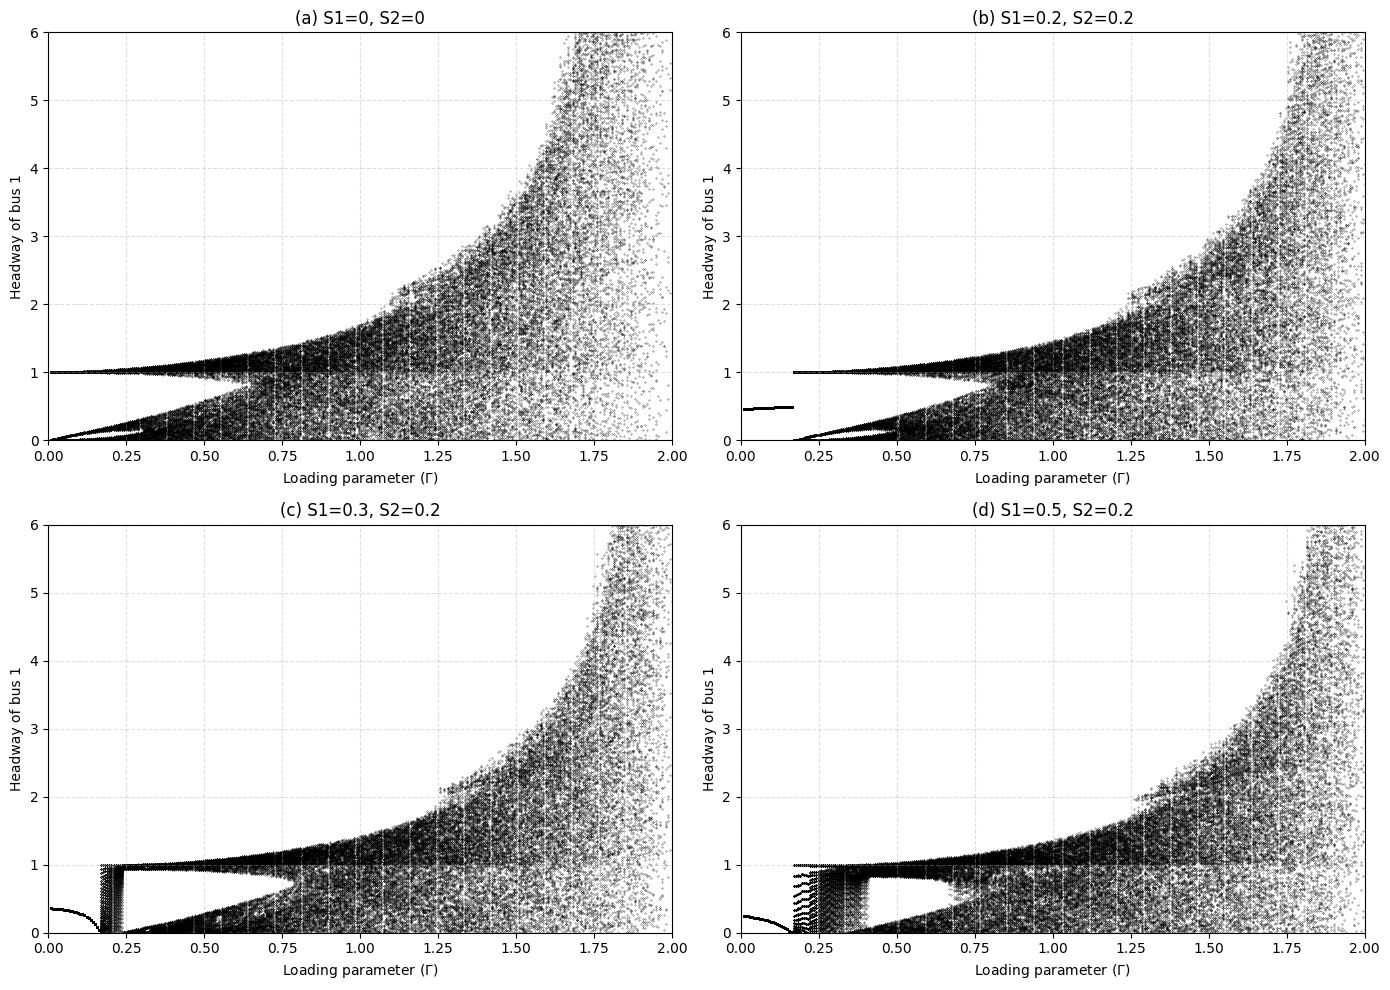
\includegraphics[width=\textwidth,height=0.43\textheight,keepaspectratio]{fig2_bifurcation.png}
    \caption{Bifurcation diagrams: $H_1(m)$ vs.\ $\Gamma$, trips 1000--1200. (a)~$S_1\!=\!S_2\!=\!0$, (b)~$S_1\!=\!S_2\!=\!0.2$, (c)~$S_1\!=\!0.3,S_2\!=\!0.2$, (d)~$S_1\!=\!0.5,S_2\!=\!0.2$.}
    \label{fig:fig2_bifurcation}
\end{figure*}

Figure~\ref{fig:fig3_zoom} zooms to $\Gamma\in[0,0.5]$, revealing the \textbf{period-adding} route to chaos: periods grow $3\to5\to7\to\cdots$ rather than doubling. This is a hallmark of piecewise-smooth maps and qualitatively distinct from period-doubling cascades. Regularity windows---brief returns to periodic orbits within the chaotic band---are visible in case (b).

\begin{figure*}[tbp]
    \centering
    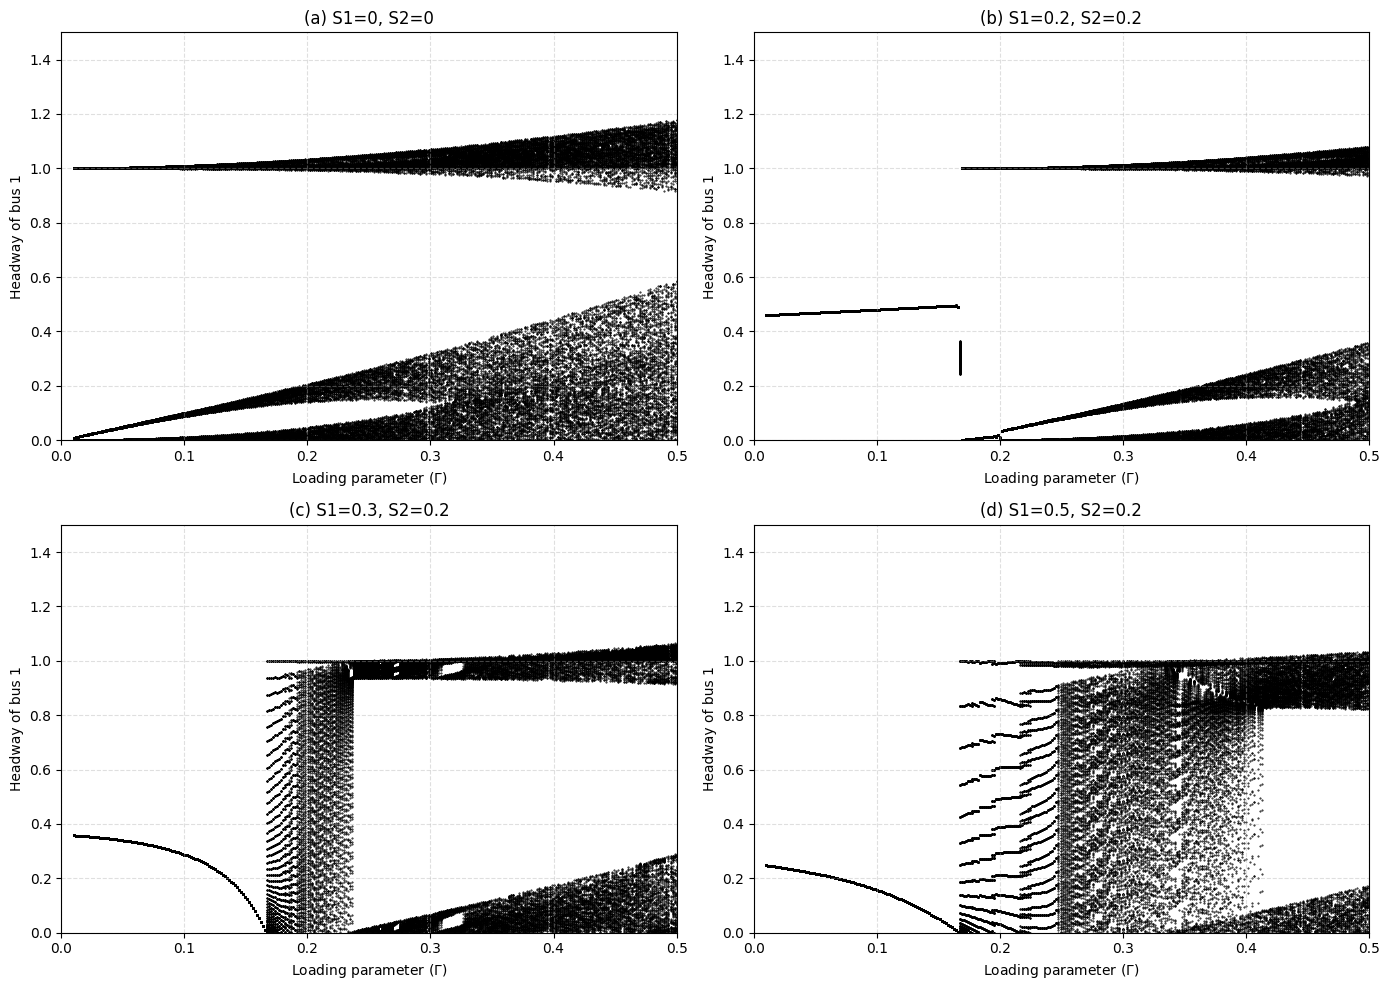
\includegraphics[width=\textwidth,height=0.43\textheight,keepaspectratio]{fig3_zoom.png}
    \caption{Zoom of Fig.~\ref{fig:fig2_bifurcation} to $0<\Gamma<0.5$, showing the period-adding bifurcation fan.}
    \label{fig:fig3_zoom}
\end{figure*}

\subsection{Tour Time Dynamics (Figs.~4--5)}

\begin{figure*}[tbp]
    \centering
    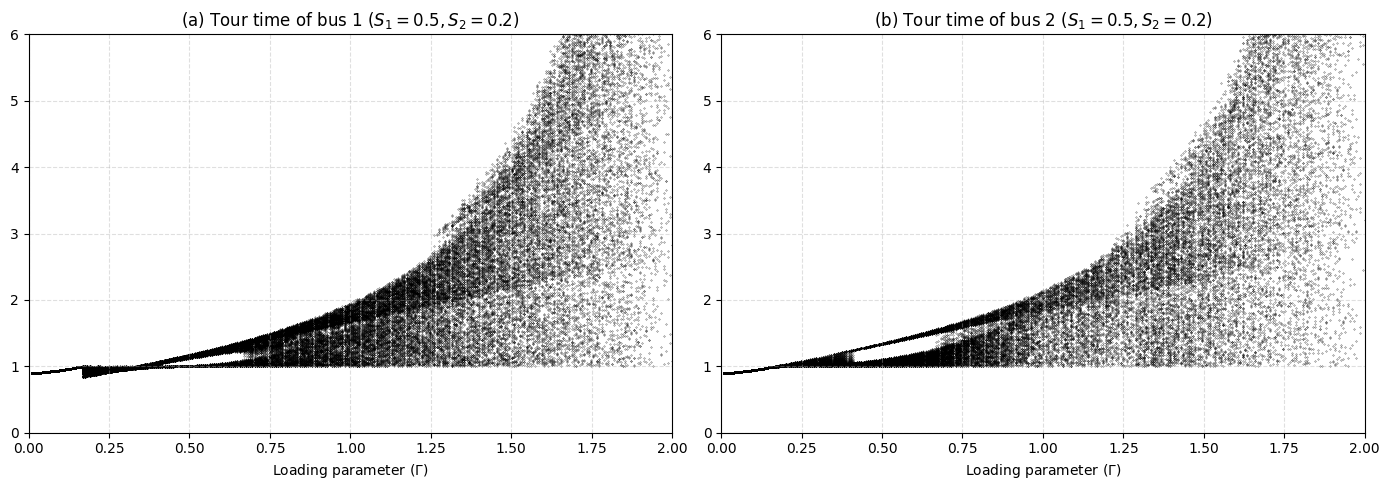
\includegraphics[width=\textwidth,height=0.30\textheight,keepaspectratio]{fig4_tour.png}
    \caption{Tour times $\Delta T_1$ (a) and $\Delta T_2$ (b) vs.\ $\Gamma$ for $S_1\!=\!0.5$, $S_2\!=\!0.2$.}
    \label{fig:fig4_tour}
\end{figure*}

Figure~\ref{fig:fig4_tour} shows tour times for $S_1=0.5$, $S_2=0.2$. Both buses are synchronised until $\Gamma\approx0.167$. Beyond that, Bus~1's stronger speedup causes larger overshoot: big headway $\to$ big speed increase $\to$ small next headway. Bus~2 reacts weakly and initially stays constrained; their amplitude roles swap at $\Gamma\approx0.333$ (Point~2 of Fig.~\ref{fig:fig7_stats}). Figure~\ref{fig:fig5_tour_zoom} confirms the transition points align exactly with the headway bifurcations.

\begin{figure*}[tbp]
    \centering
    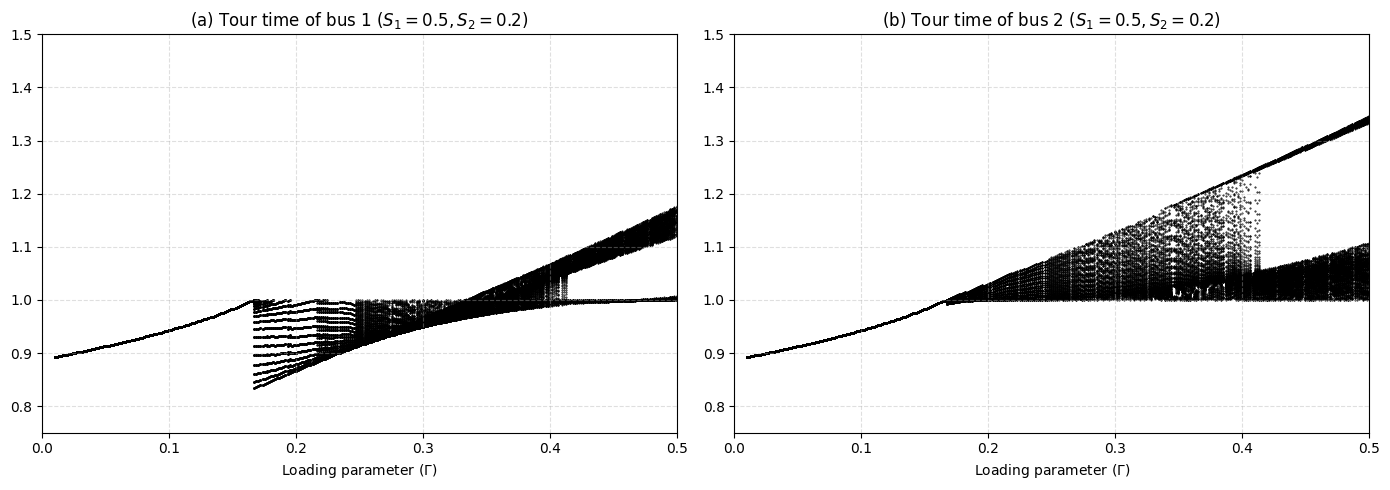
\includegraphics[width=\textwidth,height=0.30\textheight,keepaspectratio]{fig5_tour_zoom.png}
    \caption{Tour time zoom ($0<\Gamma<0.5$): transition points match headway bifurcations exactly.}
    \label{fig:fig5_tour_zoom}
\end{figure*}

\subsection{Return Maps (Fig.~6)}

\begin{figure*}[tbp]
    \centering
    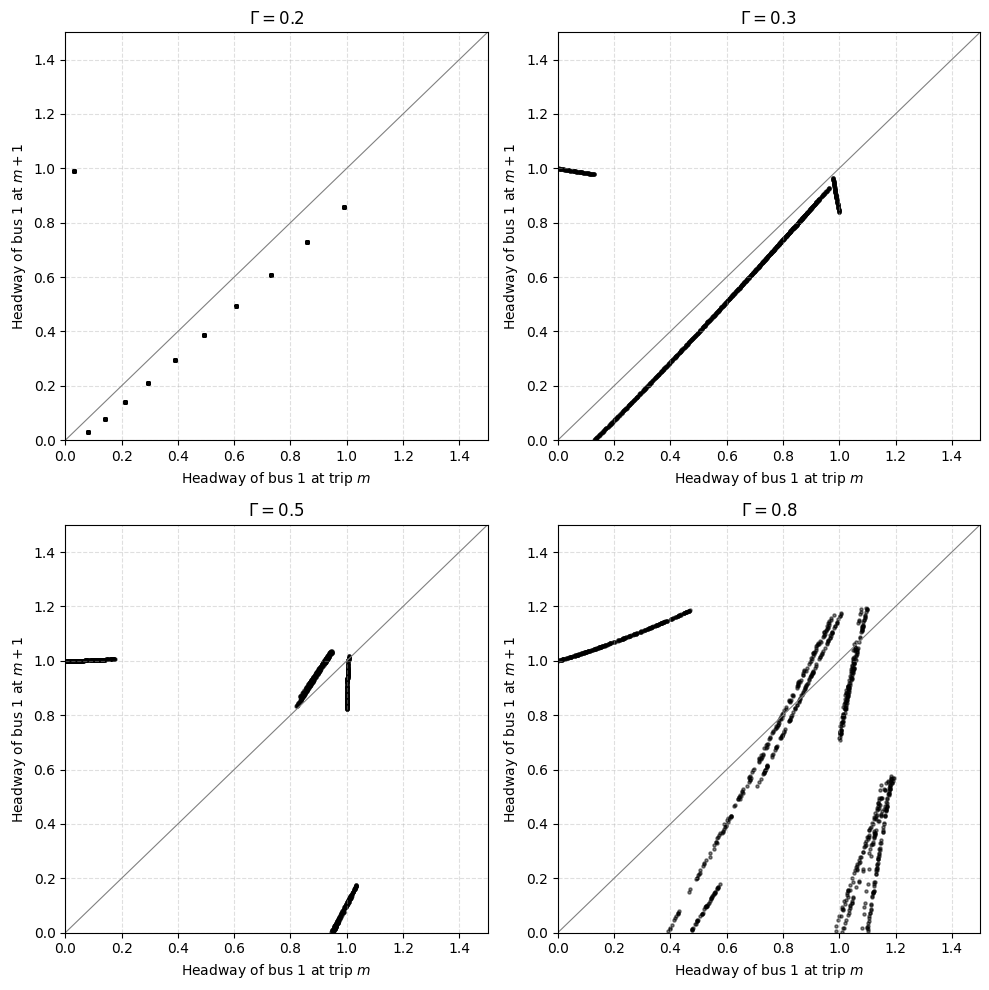
\includegraphics[width=\textwidth,height=0.43\textheight,keepaspectratio]{fig6_return_map.png}
    \caption{Return maps $H_1(m{+}1)$ vs.\ $H_1(m)$, trips 1000--2000. $S_1\!=\!0.5$, $S_2\!=\!0.2$. (a)~$\Gamma\!=\!0.2$: period-11 orbit; (b)~$\Gamma\!=\!0.3$: piecewise-linear curve; (c,d) progressive fragmentation.}
    \label{fig:fig6_return_map}
\end{figure*}

Return maps (Fig.~\ref{fig:fig6_return_map}) diagnose the regime. At $\Gamma=0.2$: exactly 11 discrete points (period-11 orbit). At $\Gamma=0.3$: a piecewise-linear curve---the hallmark of deterministic chaos; the ascending branch has slope $>1$, consistent with sensitive dependence on initial conditions. By $\Gamma=0.8$ the attractor has fragmented into multiple crossing strands. In all cases \emph{geometric structure is present}: the dynamics are governed by the nonlinear map, not by noise.

\subsection{Statistical Analysis (Fig.~7)}

\begin{figure*}[tbp]
    \centering
    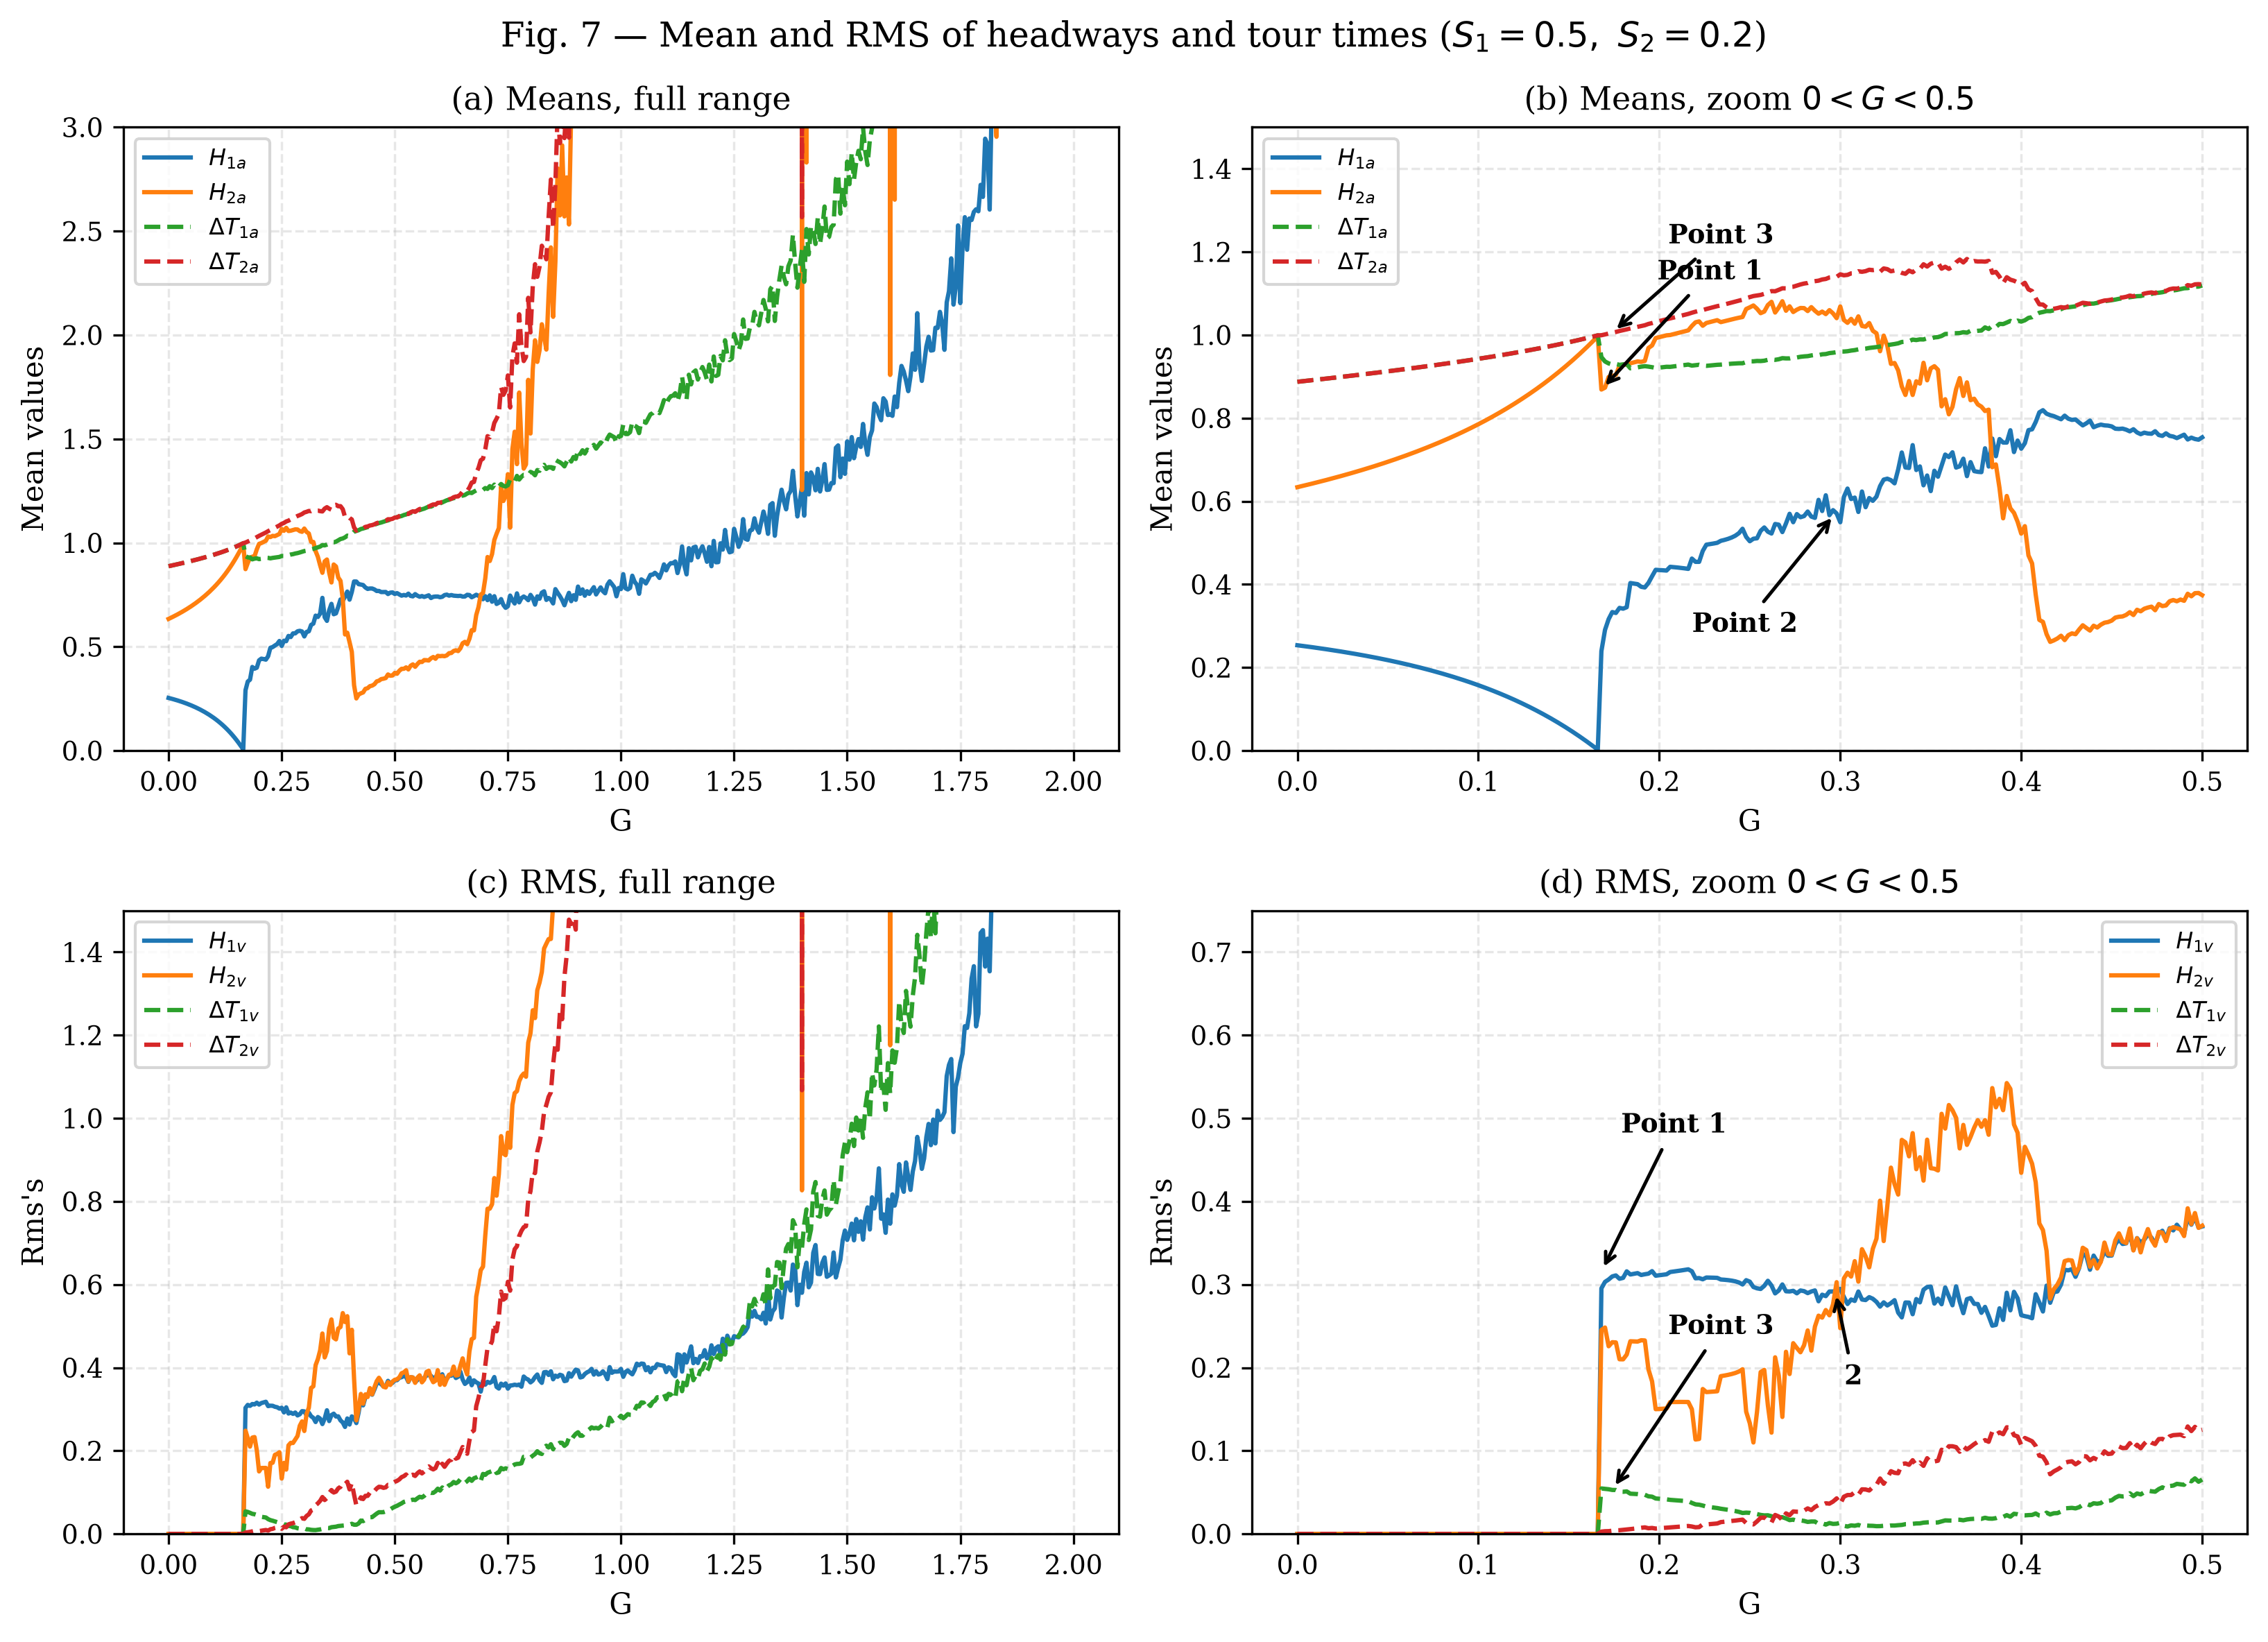
\includegraphics[width=\textwidth,height=0.43\textheight,keepaspectratio]{fig7_stats.png}
    \caption{Mean (a,b) and RMS (c,d) of headway and tour time vs.\ $\Gamma$. Insets zoom to $0<\Gamma<0.5$. Points 1, 2, 3 mark transition loadings computed numerically.}
    \label{fig:fig7_stats}
\end{figure*}

Figure~\ref{fig:fig7_stats}: RMS is zero for $\Gamma<0.167$ (regular) and jumps sharply at \textbf{Point 1} ($\Gamma\approx0.167$). Past Point~1, Bus~2's mean headway ($S_2=0.2$, weaker correction) drops sharply toward zero while Bus~1's rises---Bus~2 is closer to bunching. Means cross at \textbf{Point 2} ($\Gamma\approx0.333$). \textbf{Point 3} ($\Gamma\approx0.407$) marks the tour-time RMS minimum. Near-vertical spikes above $\Gamma\approx1.3$ are resonance windows where the system briefly re-synchronises.

% ─────────────────────────────────────────────────────────────────────────────
\section{Phase Diagram and Analysis}

\subsection{Phase Boundary $\Gamma^*(S)$ (Fig.~8)}

\begin{figure}[htbp]
    \centering
    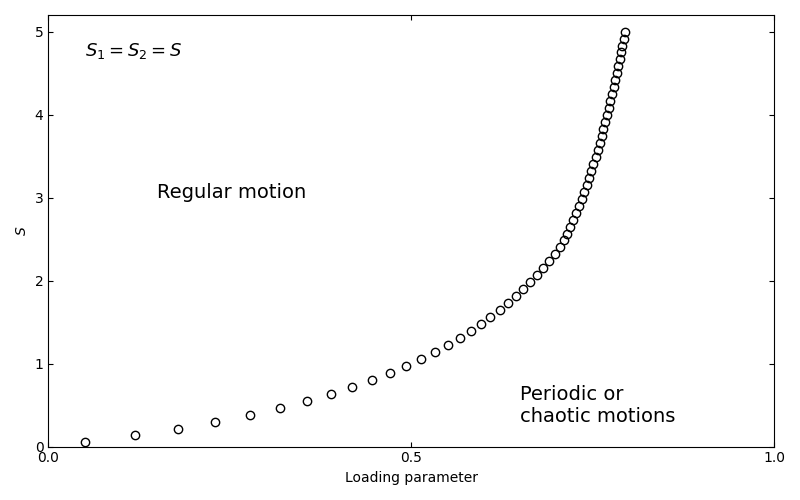
\includegraphics[width=\columnwidth]{fig8_phase_diagram.png}
    \caption{Phase diagram: numerically determined boundary $\Gamma^*(S)$ for $S_1\!=\!S_2\!=\!S$ by bisection. Above the curve: regular motion; below: periodic/chaotic.}
    \label{fig:fig8_phase_diagram}
\end{figure}

We locate $\Gamma^*(S)$ by bisection search on $\Gamma$ for each symmetric speedup $S_1=S_2=S$, using an RMS threshold to detect chaos. The boundary (Fig.~\ref{fig:fig8_phase_diagram}) is concave-upward: early units of speedup yield diminishing returns in expanding the safe loading range. Section~\ref{sec:ext} shows this curve terminates at a finite $S_c$ beyond which the system is chaotic even at $\Gamma=0$.

\subsection{Limitations}

The model assumes constant $\mu$, linear dwell times, and no traffic noise. The RMS classification cannot distinguish high-period periodic orbits from broadband chaos; a rigorous separation requires return-map inspection (Fig.~\ref{fig:fig6_return_map}) or Lyapunov exponent computation, neither of which we automate.

\subsection{Sensitivity to Initial Conditions}

\begin{figure*}[tbp]
    \centering
    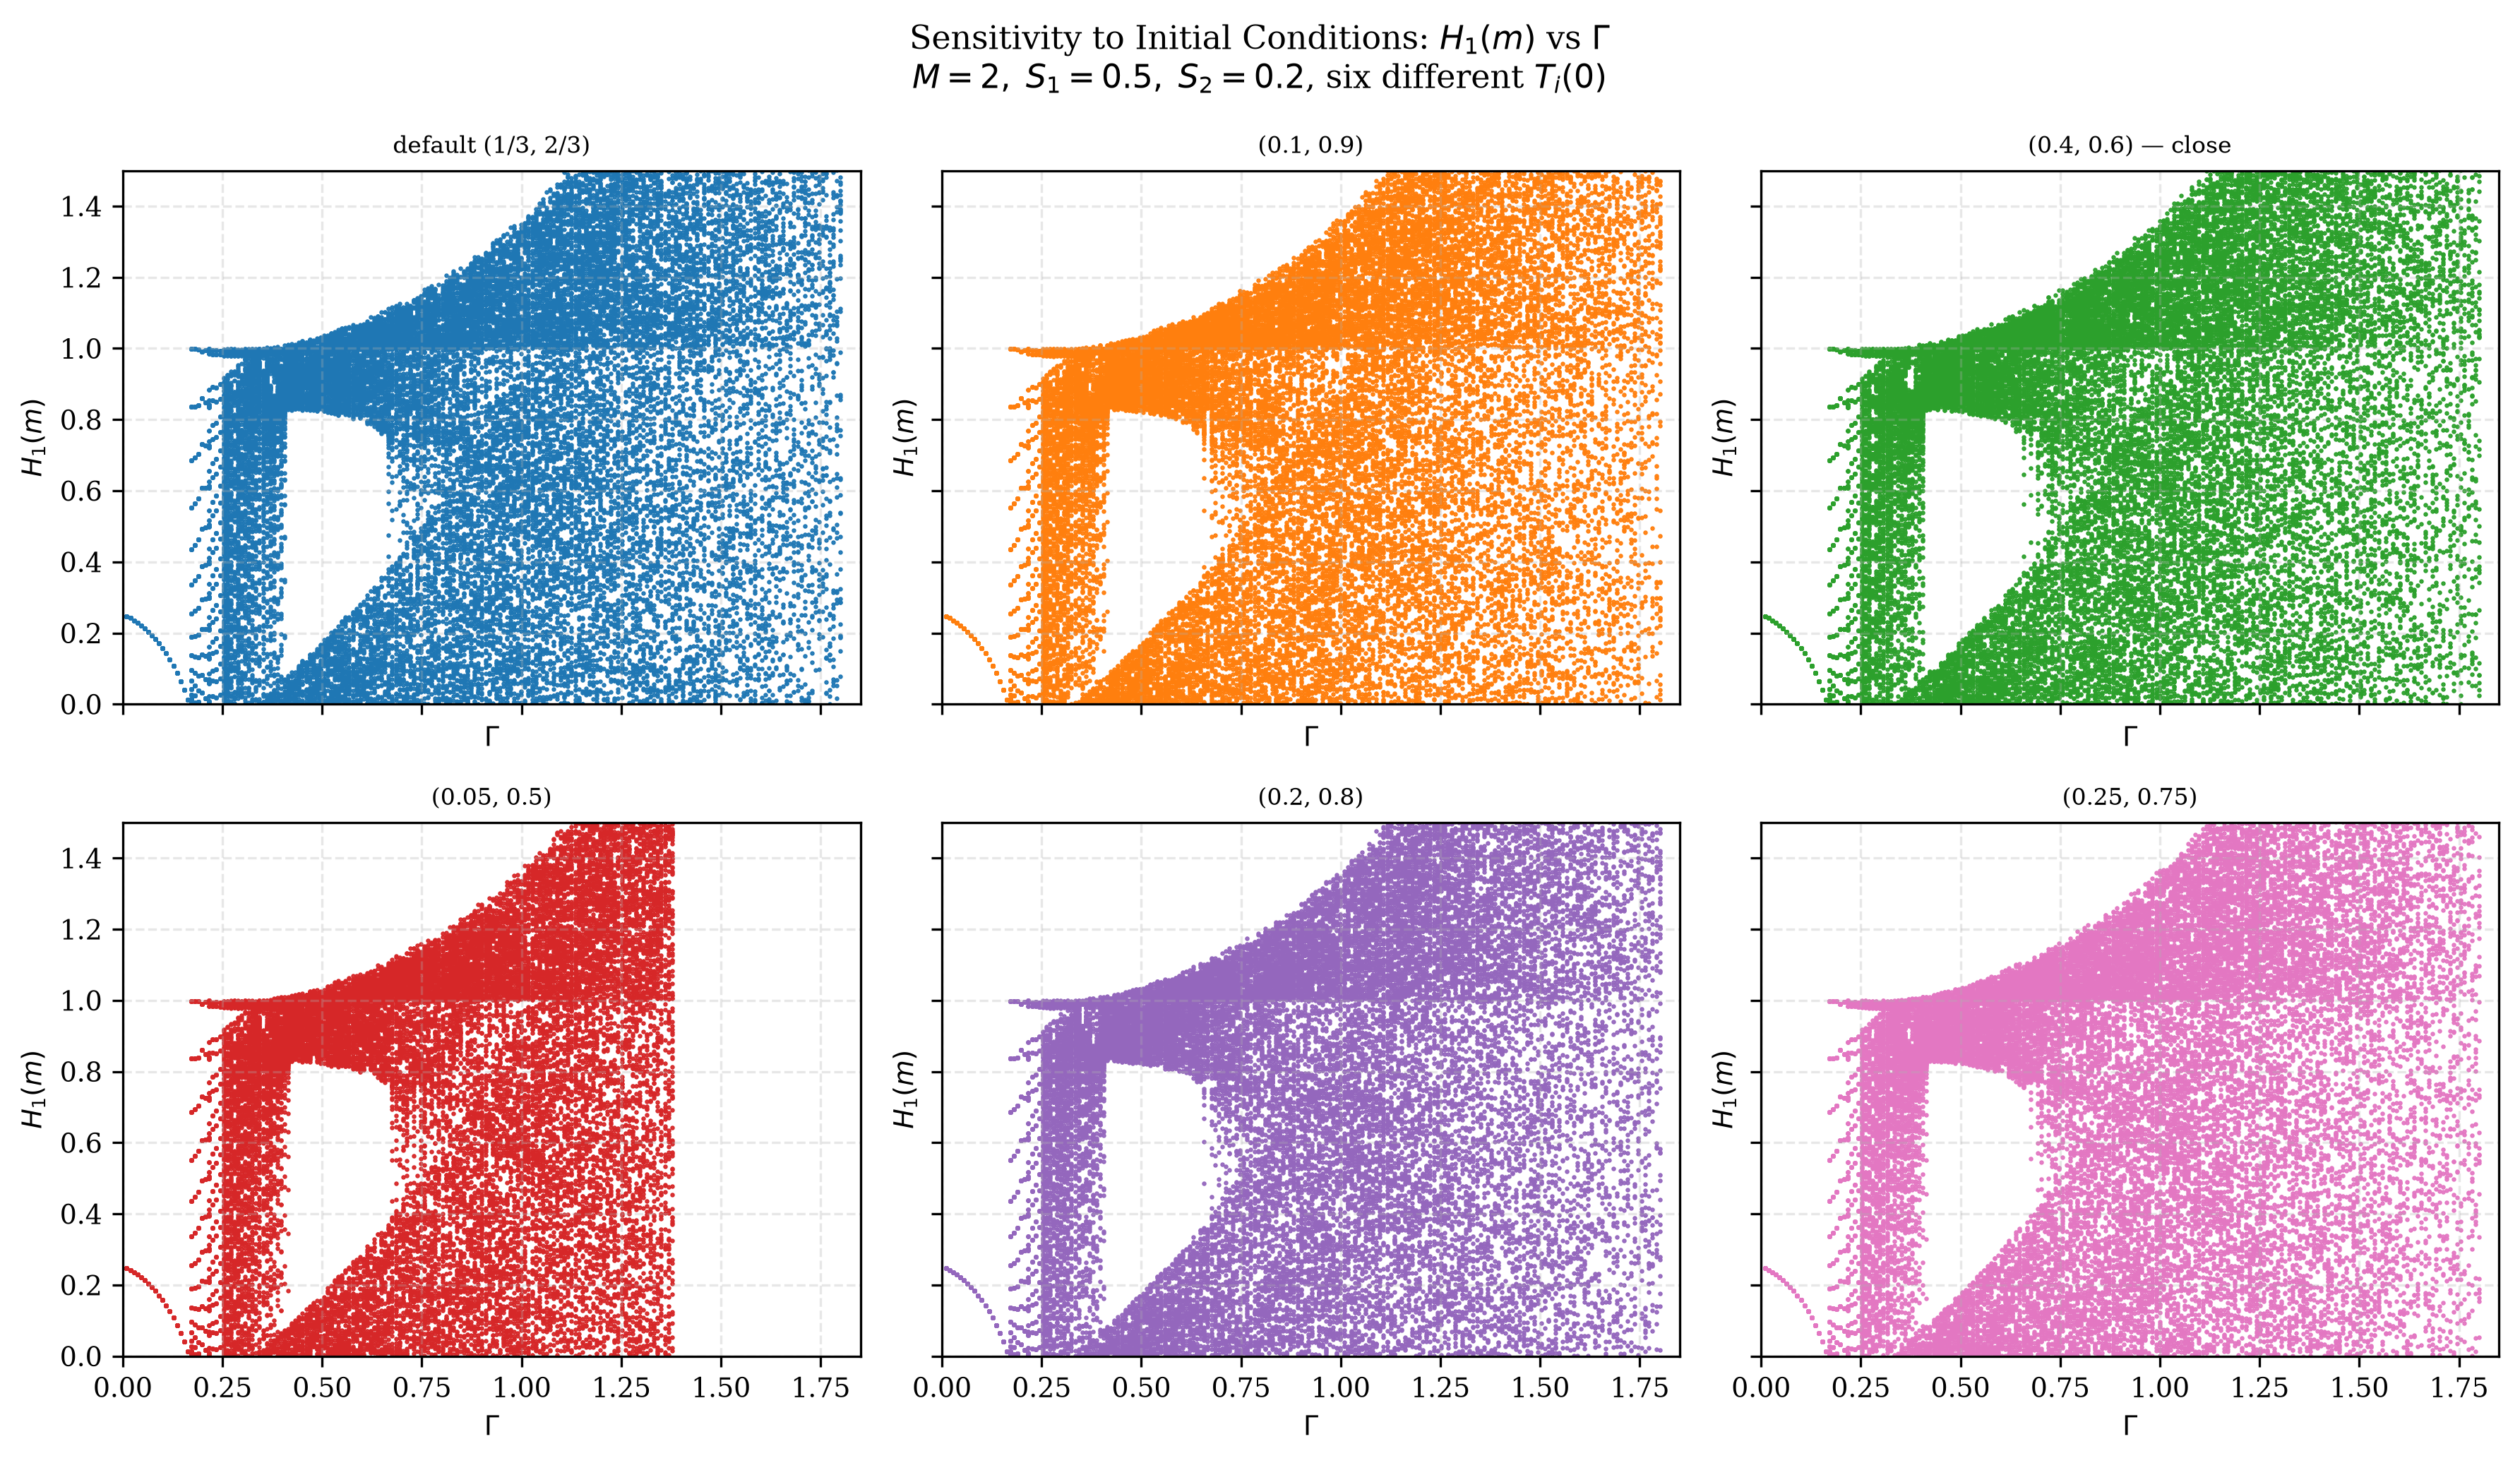
\includegraphics[width=\textwidth,height=0.42\textheight,keepaspectratio]{fig_sensitivity_ic.png}
    \caption{Bifurcation diagrams from six different initial conditions $(T_1(0),T_2(0))$. All panels are visually identical: the attractor is unique and independent of initial configuration after 1000-trip transient elimination.}
    \label{fig:sensitivity_ic}
\end{figure*}

Figure~\ref{fig:sensitivity_ic} overlays bifurcation diagrams from six initial-condition pairs ranging from nearly equal $(0.4,0.6)$ to strongly asymmetric $(0.05,0.5)$. All six are visually indistinguishable: the same period-adding windows and chaotic bands appear at identical $\Gamma$ values. This confirms (i) 1000 trips is sufficient for transient decay, and (ii) the attractor is unique---no coexisting attractors exist for the paper's parameter set.

\subsection{Robustness to Noise}

\begin{figure*}[tbp]
    \centering
    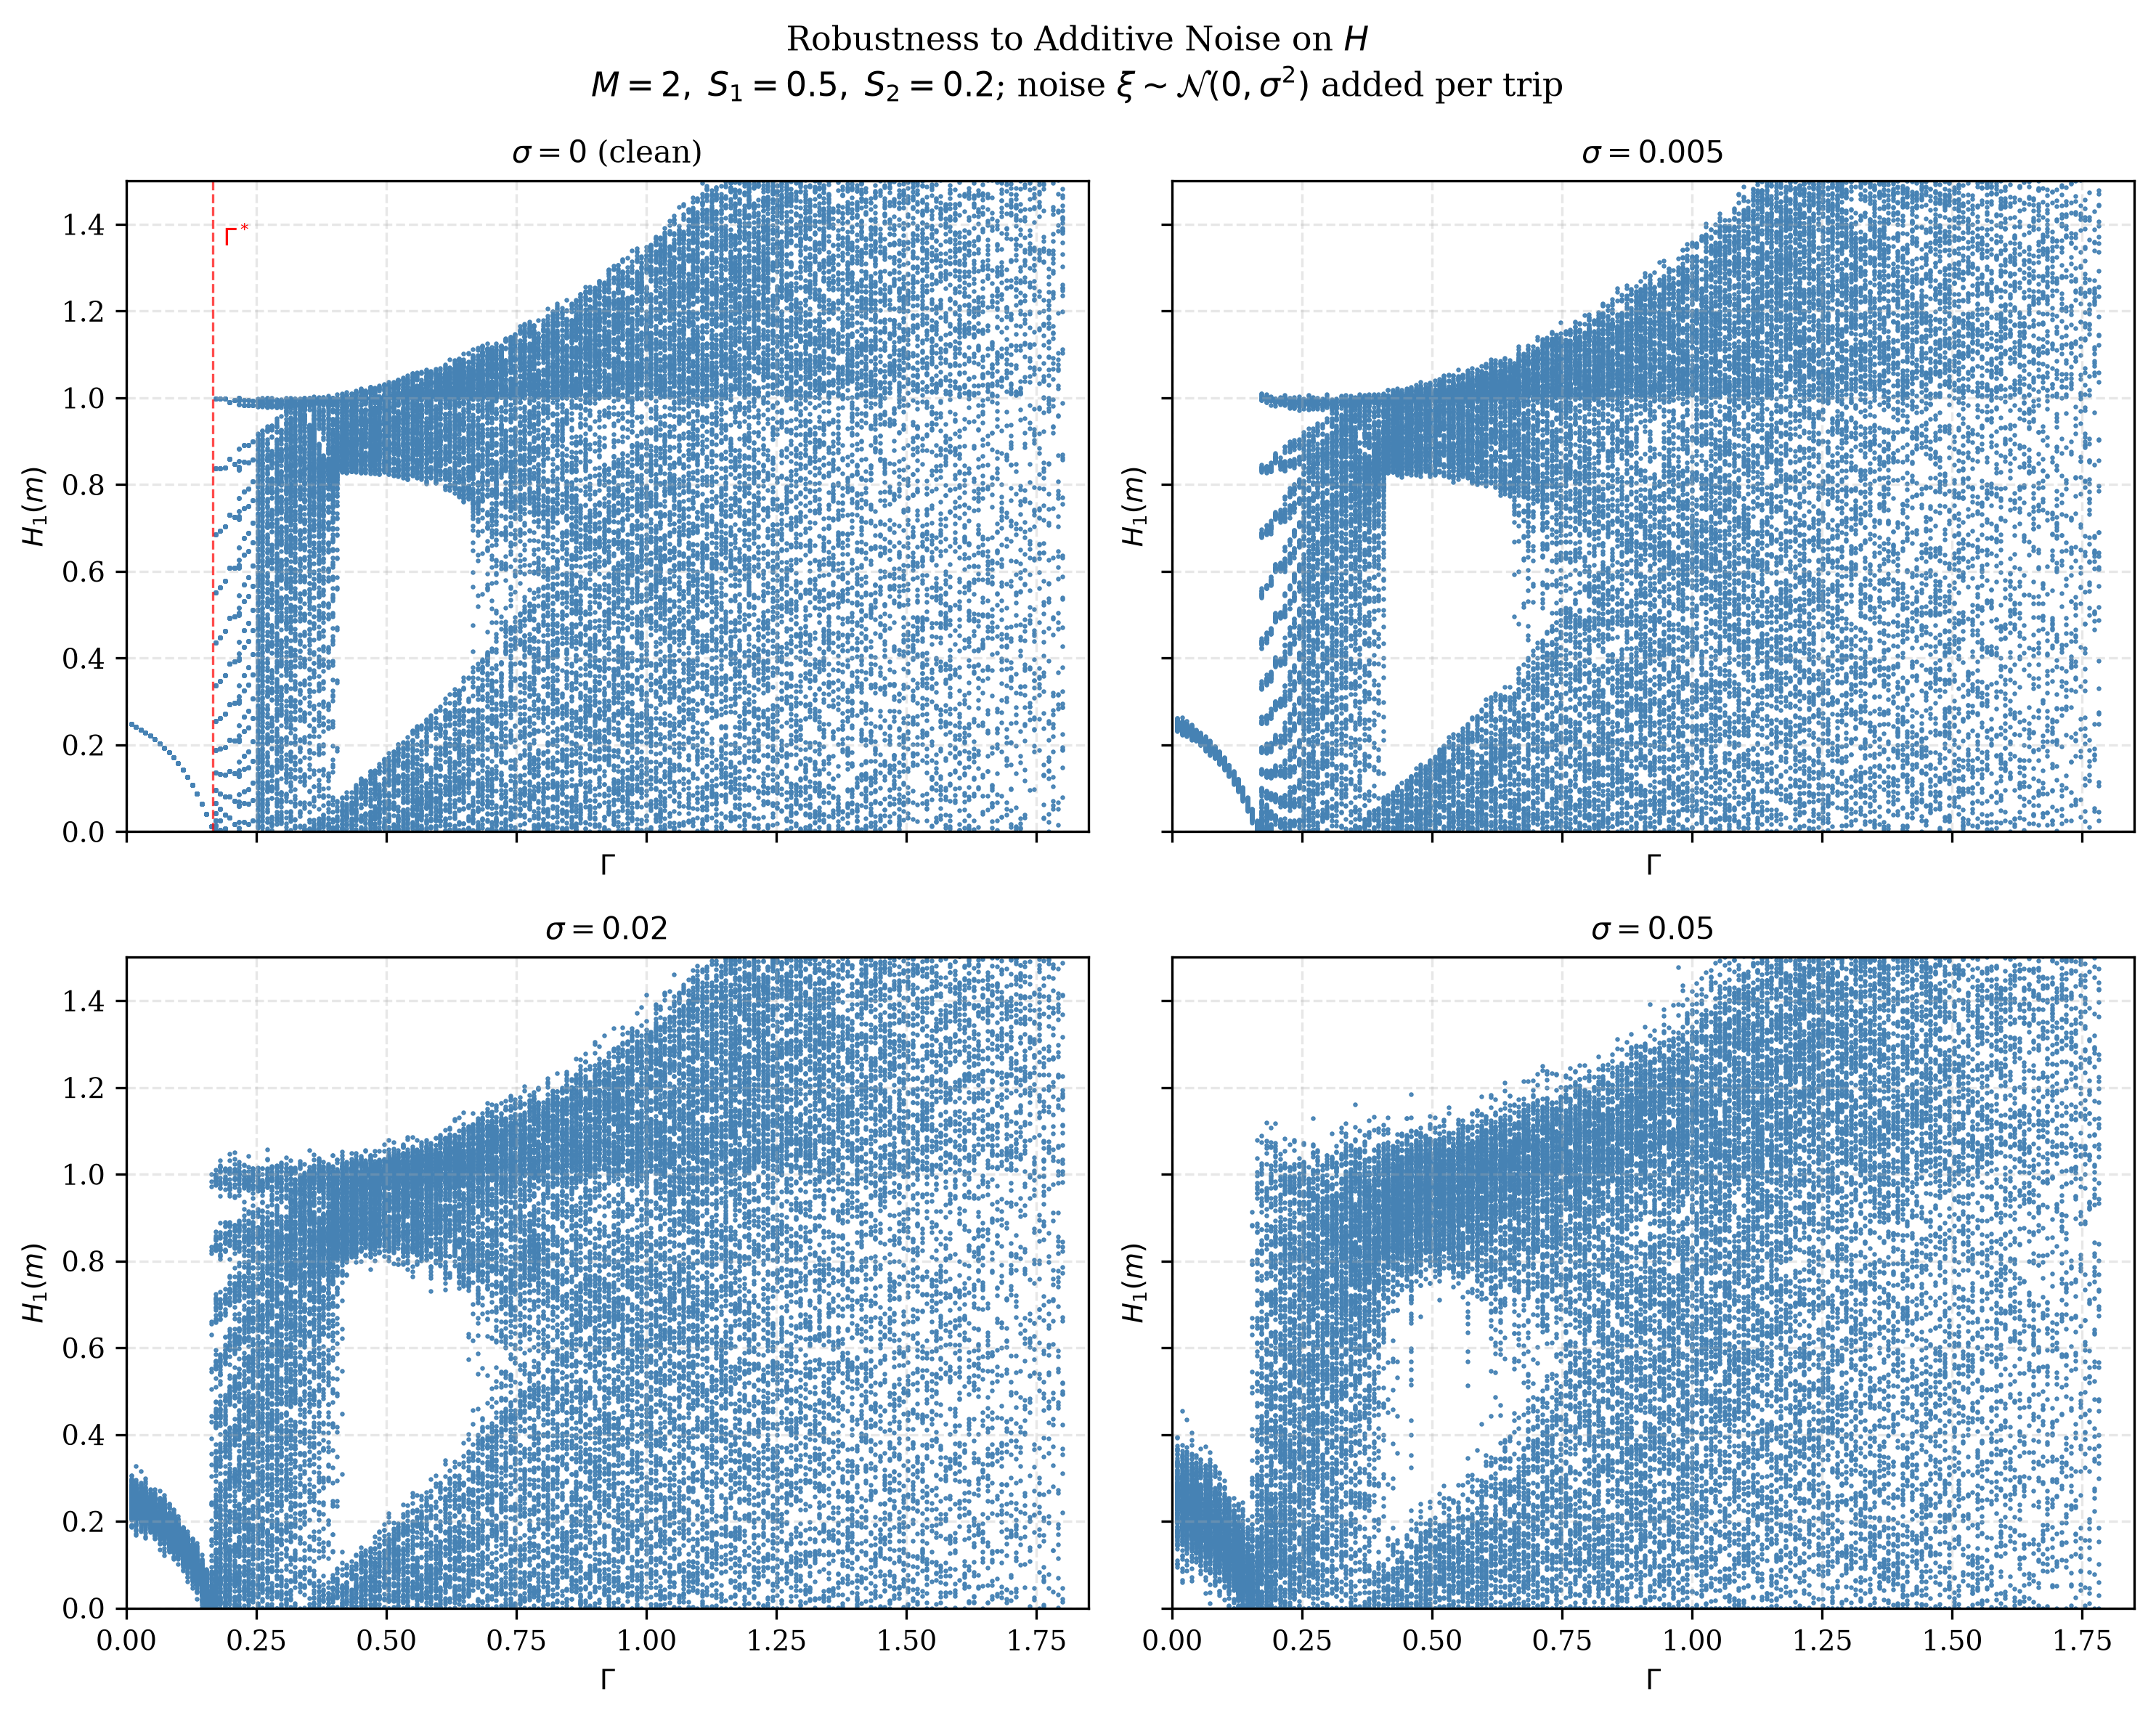
\includegraphics[width=\textwidth,height=0.37\textheight,keepaspectratio]{fig_sensitivity_noise.png}
    \caption{Bifurcation diagrams under additive noise $\xi\sim\mathcal{N}(0,\sigma^2)$ on $H$ per trip. Left to right: $\sigma=0,\,0.005,\,0.02,\,0.05$ (0--5\% of mean headway). Chaos persists at all levels; fine periodic windows erode first.}
    \label{fig:sensitivity_noise}
\end{figure*}

We add $\xi_m\sim\mathcal{N}(0,\sigma^2)$ to $H$ each trip before evaluating Eq.~\eqref{eq:final_map}, modelling per-trip timing uncertainty. Three findings from Fig.~\ref{fig:sensitivity_noise}:
\begin{enumerate}[leftmargin=*,itemsep=0pt,topsep=2pt]
    \item \textbf{Chaotic regime is robust.} Even at $\sigma=0.05$ (5\% noise) the broad headway scatter above $\Gamma^*$ persists unchanged. Noise fills the attractor but does not destroy it.
    \item \textbf{$\Gamma^*$ is stable.} The transition point does not visibly shift between $\sigma=0$ and $\sigma=0.05$: the positive-feedback instability is too strong to suppress with small perturbations.
    \item \textbf{Periodic windows erode first.} Fine-scale period-adding windows (high-period orbits with narrow basins) blur already at $\sigma=0.005$; by $\sigma=0.02$ they merge into the chaotic band. In real systems one would observe a gradual onset rather than the discrete $3\to5\to7$ sequence.
\end{enumerate}

% ─────────────────────────────────────────────────────────────────────────────
\section{Extension: $M=3$ Buses}
\label{sec:ext}

Generalising to $M=3$ requires \textbf{no new model}: Eq.~\eqref{eq:final_map} is iterated verbatim; the only change is that $i'$ is selected from two other buses instead of one. No new parameter beyond $S_3$ is introduced, and the simulation algorithm is unchanged.

\subsection{Bifurcation Diagrams (Fig.~9)}

\begin{figure*}[tbp]
    \centering
    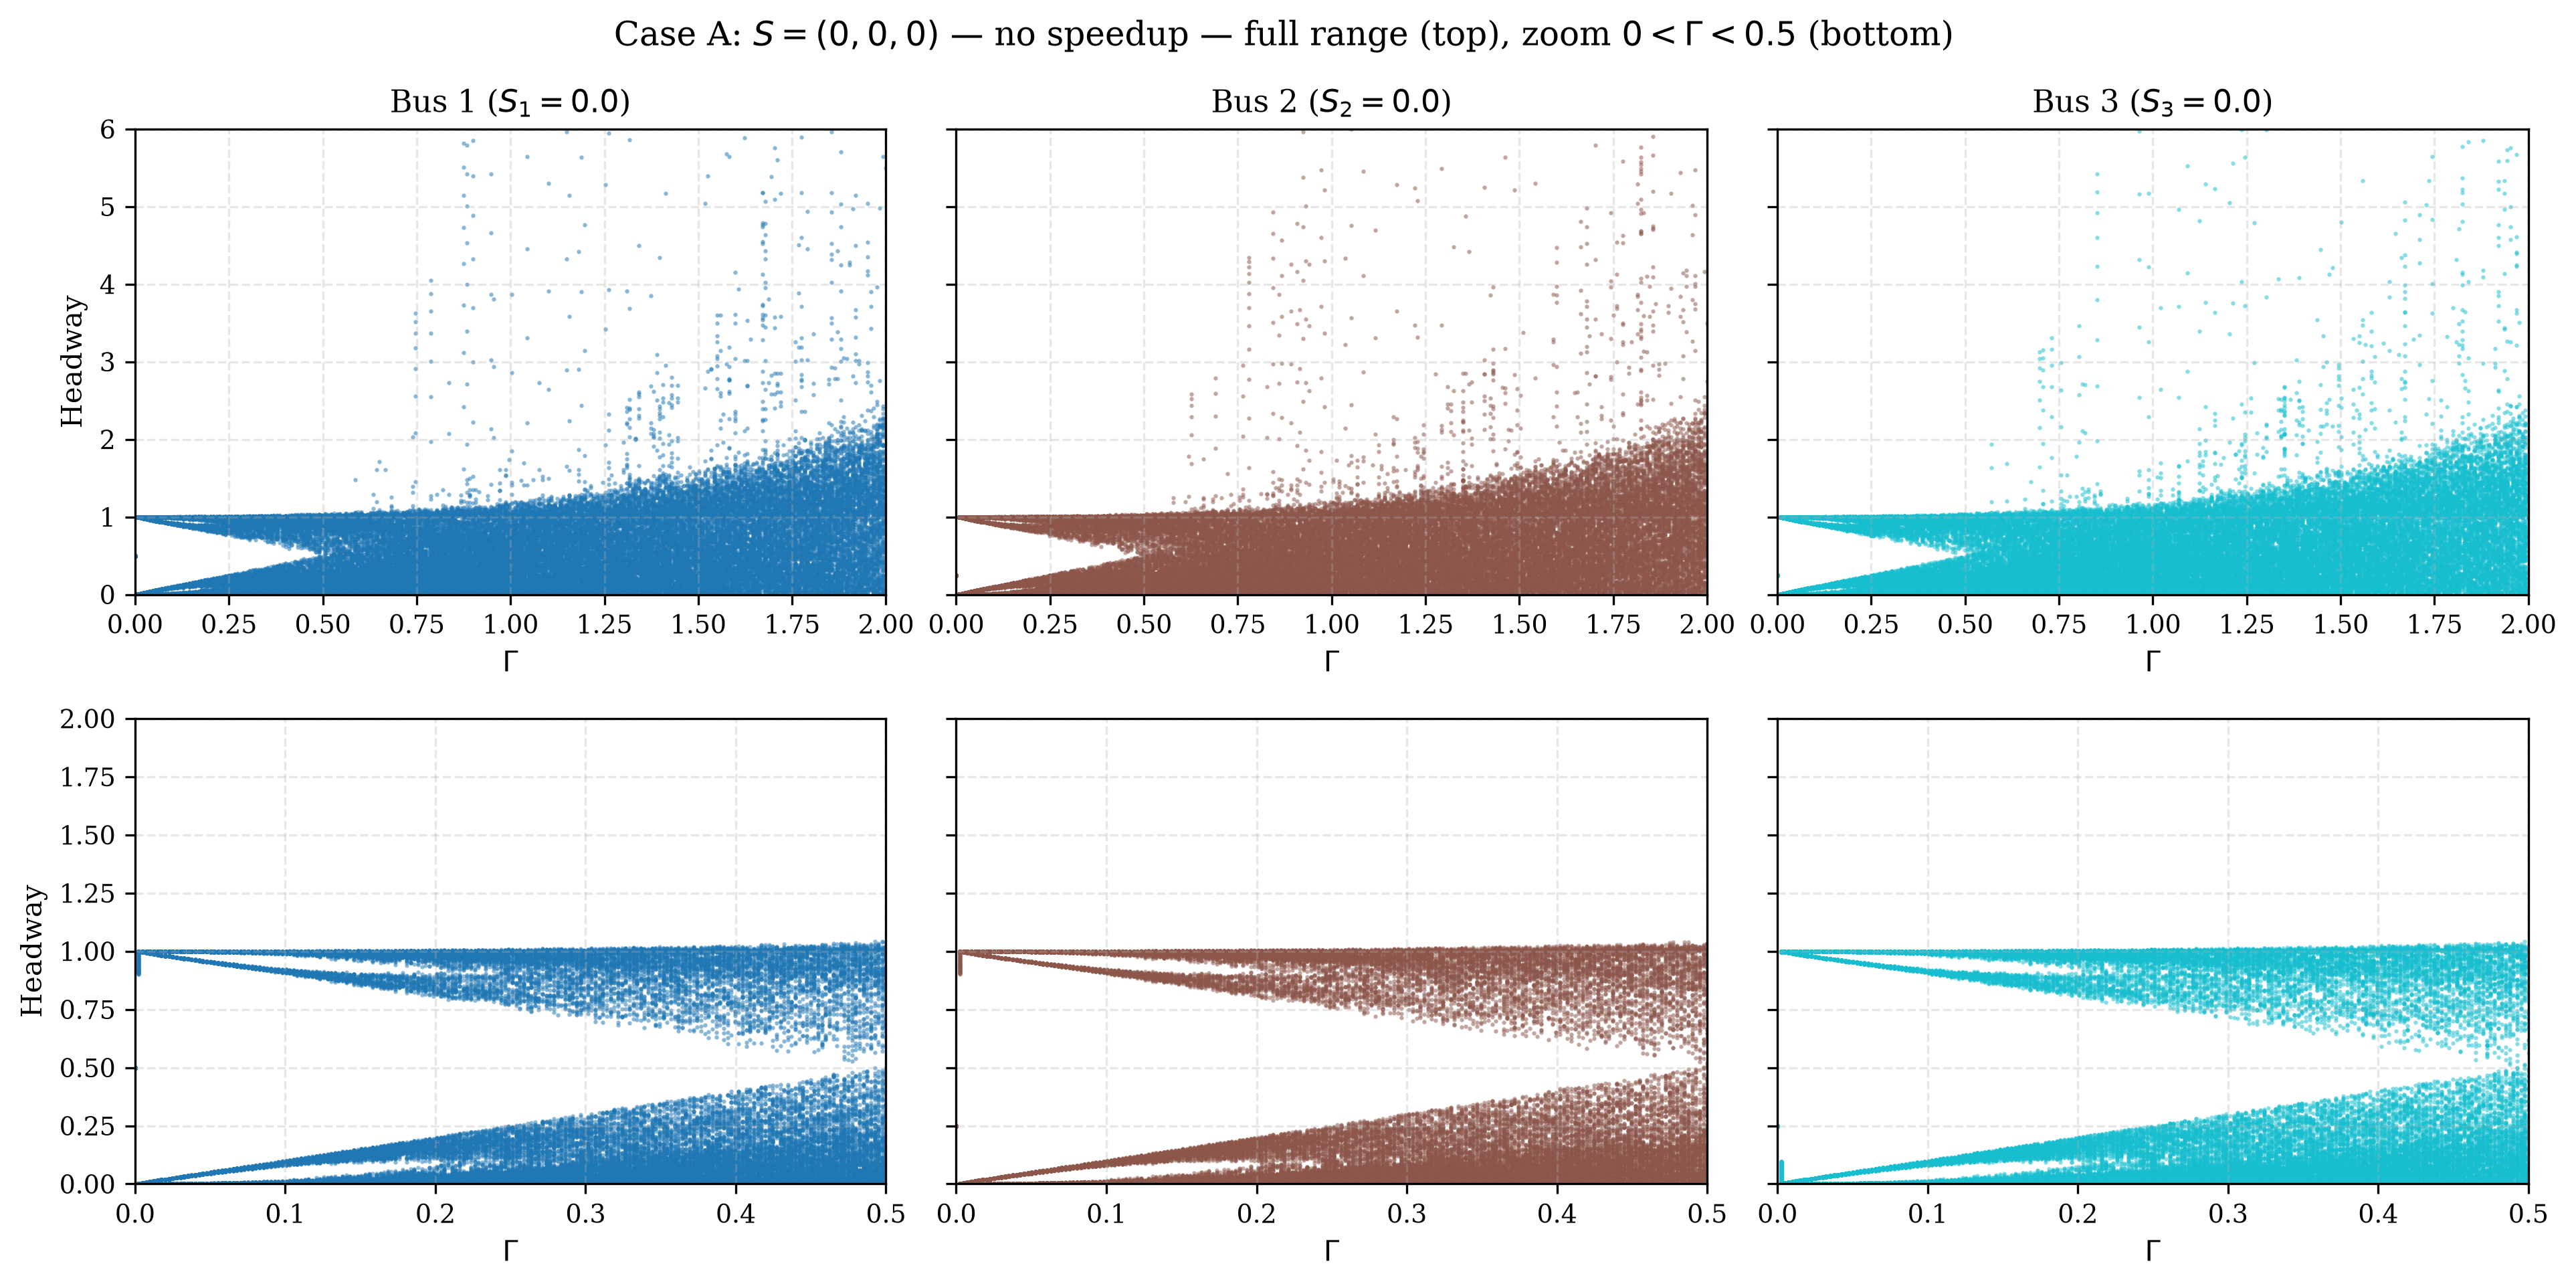
\includegraphics[width=0.49\textwidth,height=0.34\textheight,keepaspectratio]{fig9a_three_bus_S0.png}\hfill
    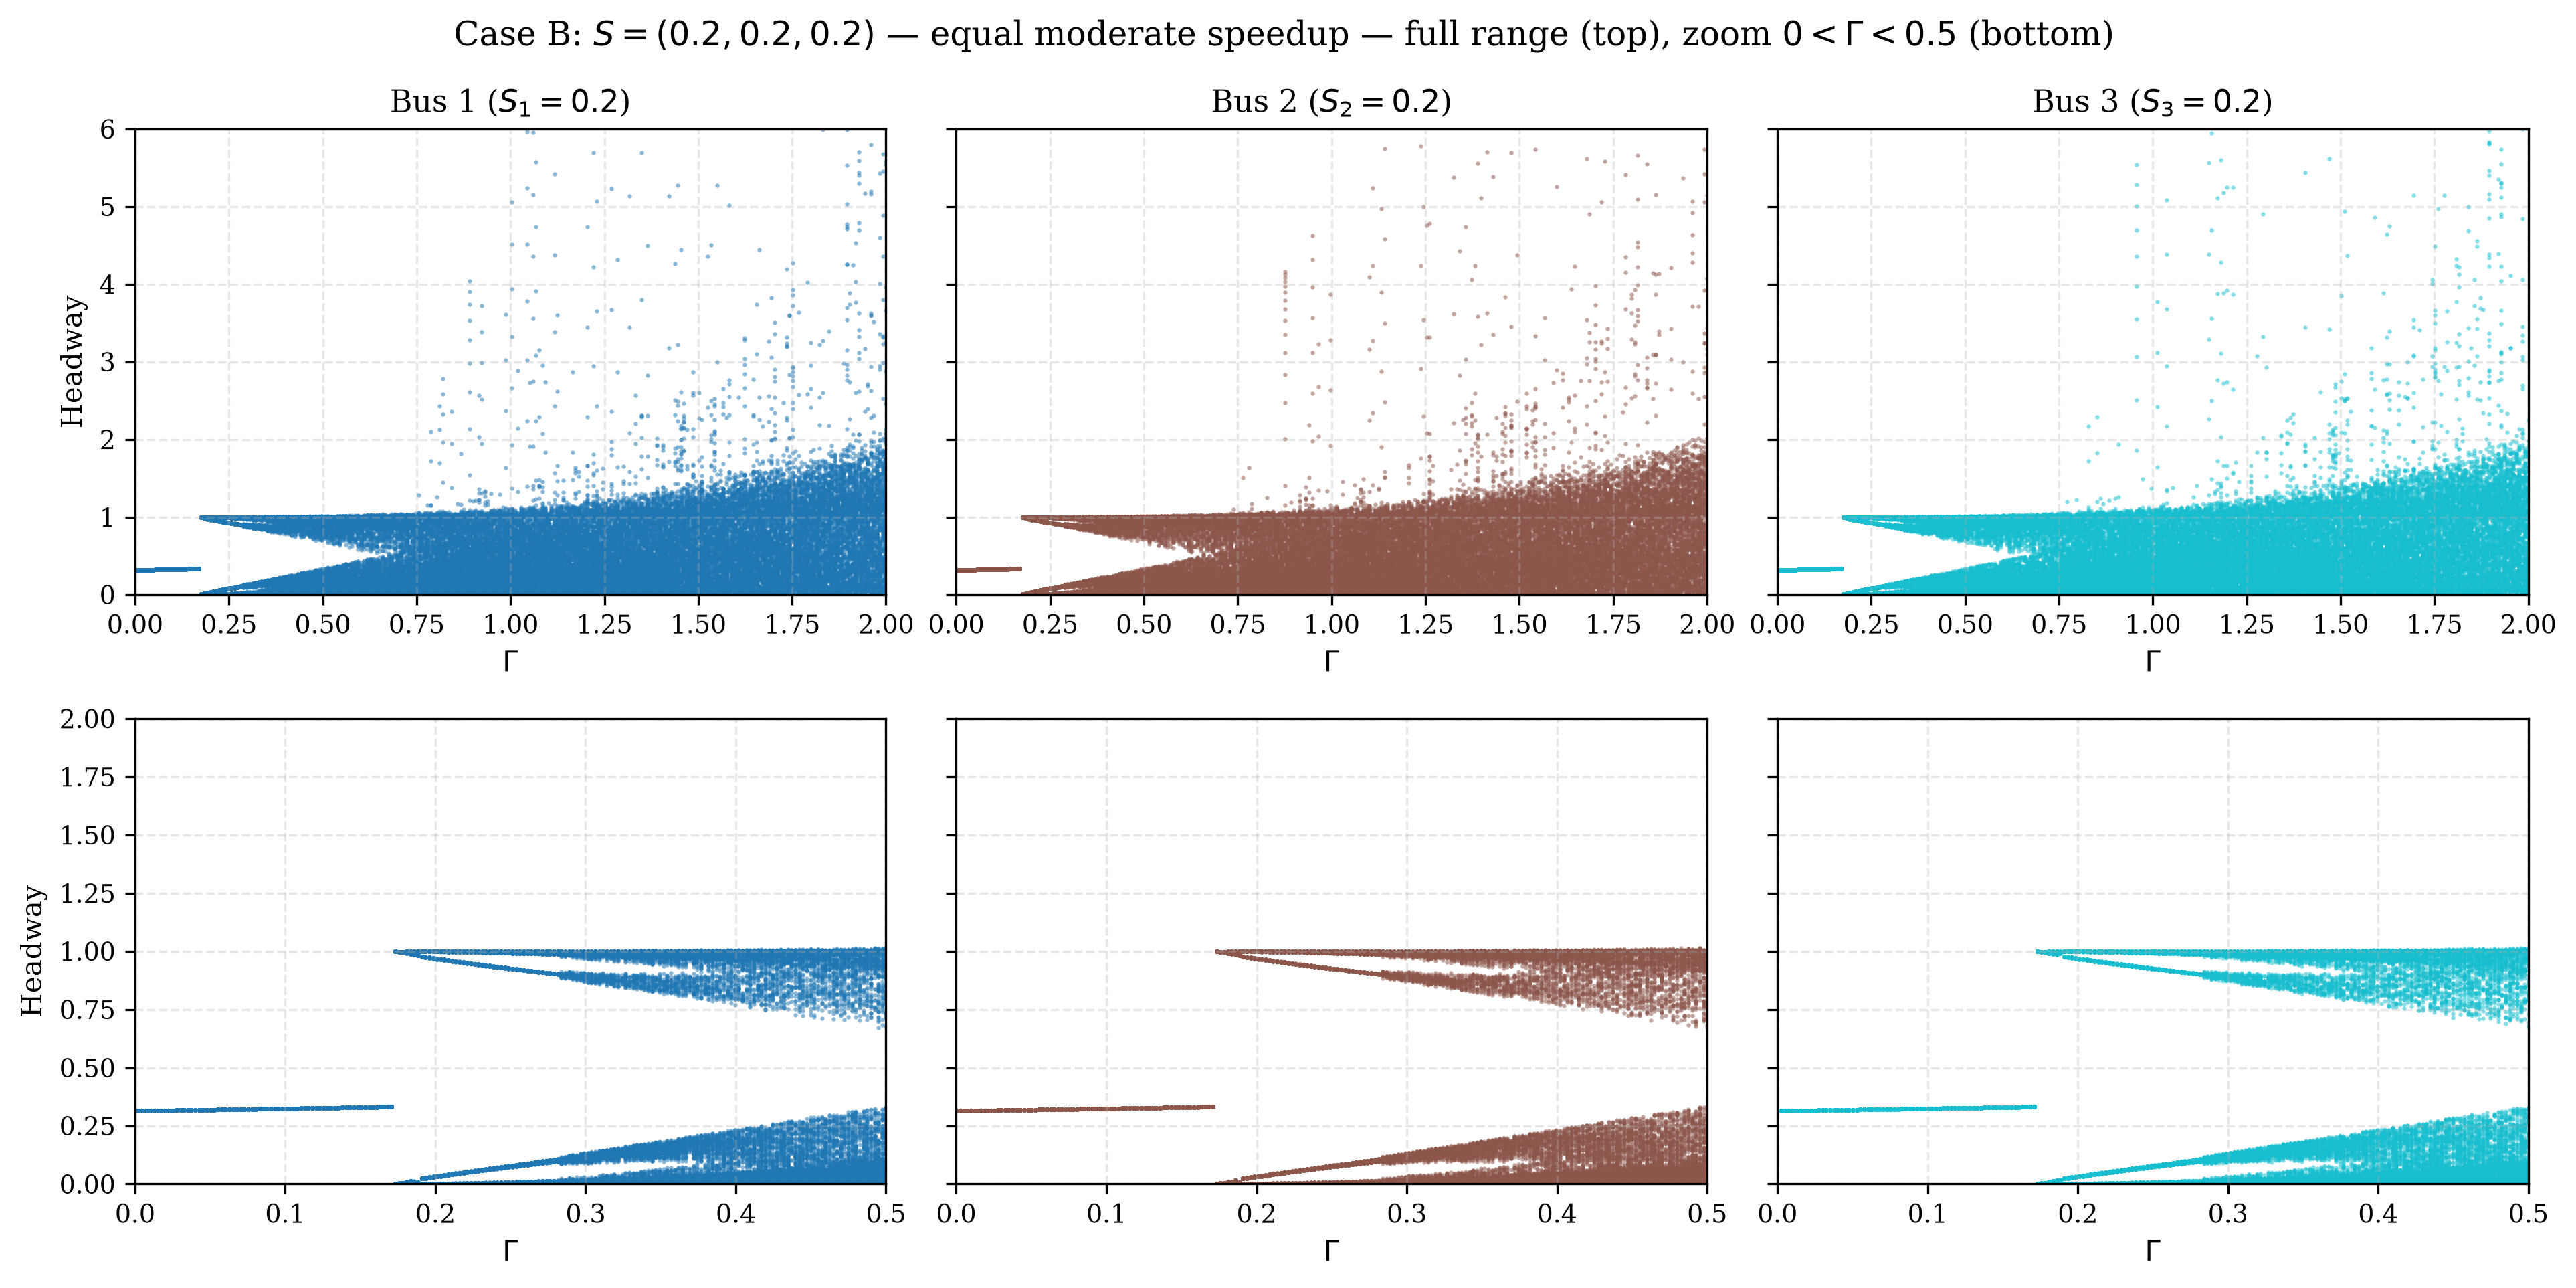
\includegraphics[width=0.49\textwidth,height=0.34\textheight,keepaspectratio]{fig9b_three_bus_S0.2.png}
    \caption{Left — Case A ($S=(0,0,0)$): no stable regime at any $\Gamma>0$.
    Right — Case B ($S=(0.2,0.2,0.2)$): shared bifurcation at $\Gamma^*=0.1733$ vs.\ $0.1685$ for $M=2$ (shift $<0.005$).}
    \label{fig:fig9a_three_bus}\label{fig:fig9b_three_bus}
\end{figure*}

\begin{figure*}[tbp]
    \centering
    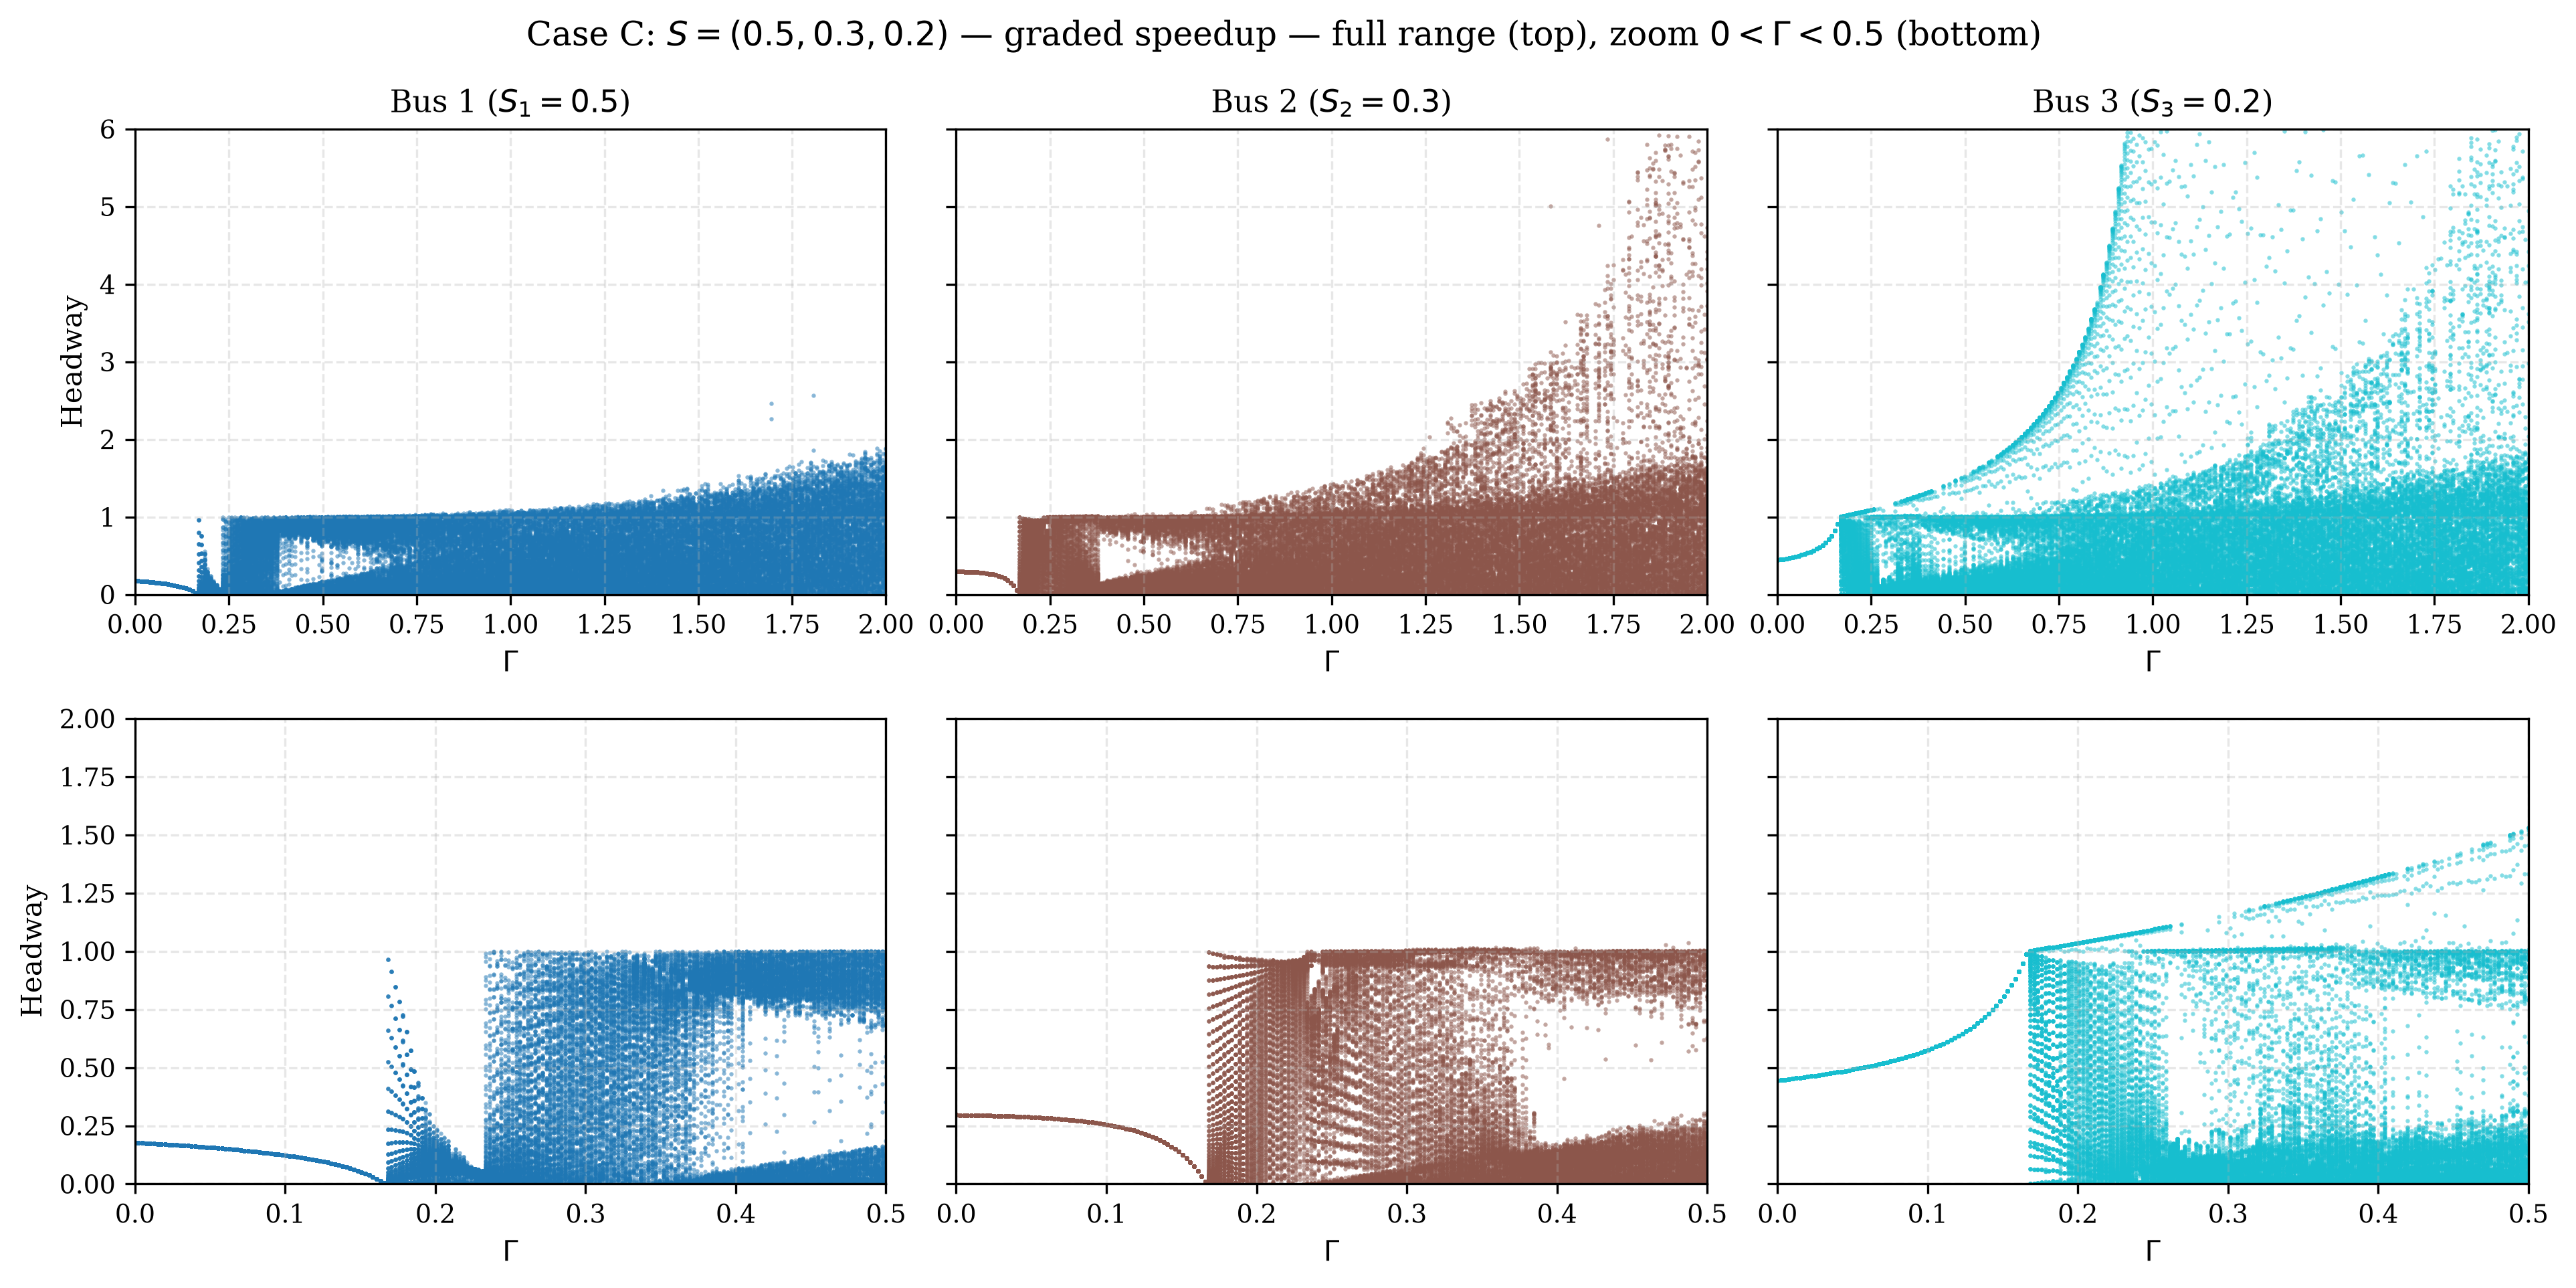
\includegraphics[width=\textwidth,height=0.34\textheight,keepaspectratio]{fig9c_three_bus_graded.png}
    \caption{Case C ($S=(0.5,0.3,0.2)$): graded speedup; weakest bus fluctuates most, same qualitative picture as Fig.~\ref{fig:fig2_bifurcation}(d).}
    \label{fig:fig9c_three_bus}
\end{figure*}

Three cases directly parallel the $M=2$ study. \textbf{Case A} ($S=(0,0,0)$, Fig.~\ref{fig:fig9a_three_bus}): no regularity at any $\Gamma$. \textbf{Case B} ($S=(0.2,0.2,0.2)$, Fig.~\ref{fig:fig9b_three_bus}): symmetric bifurcation at $\Gamma^*=0.1733$ vs.\ $\Gamma^*=0.1685$ for $M=2$---negligible shift. \textbf{Case C} ($S=(0.5,0.3,0.2)$, Fig.~\ref{fig:fig9c_three_bus}): graded response; weakest bus fluctuates most, qualitatively identical to the two-bus asymmetric case. The period-adding $3\to5\to7$ cascade is present in all cases.

\subsection{Return Maps Become Two-Valued (Fig.~10)}

\begin{figure*}[tbp]
    \centering
    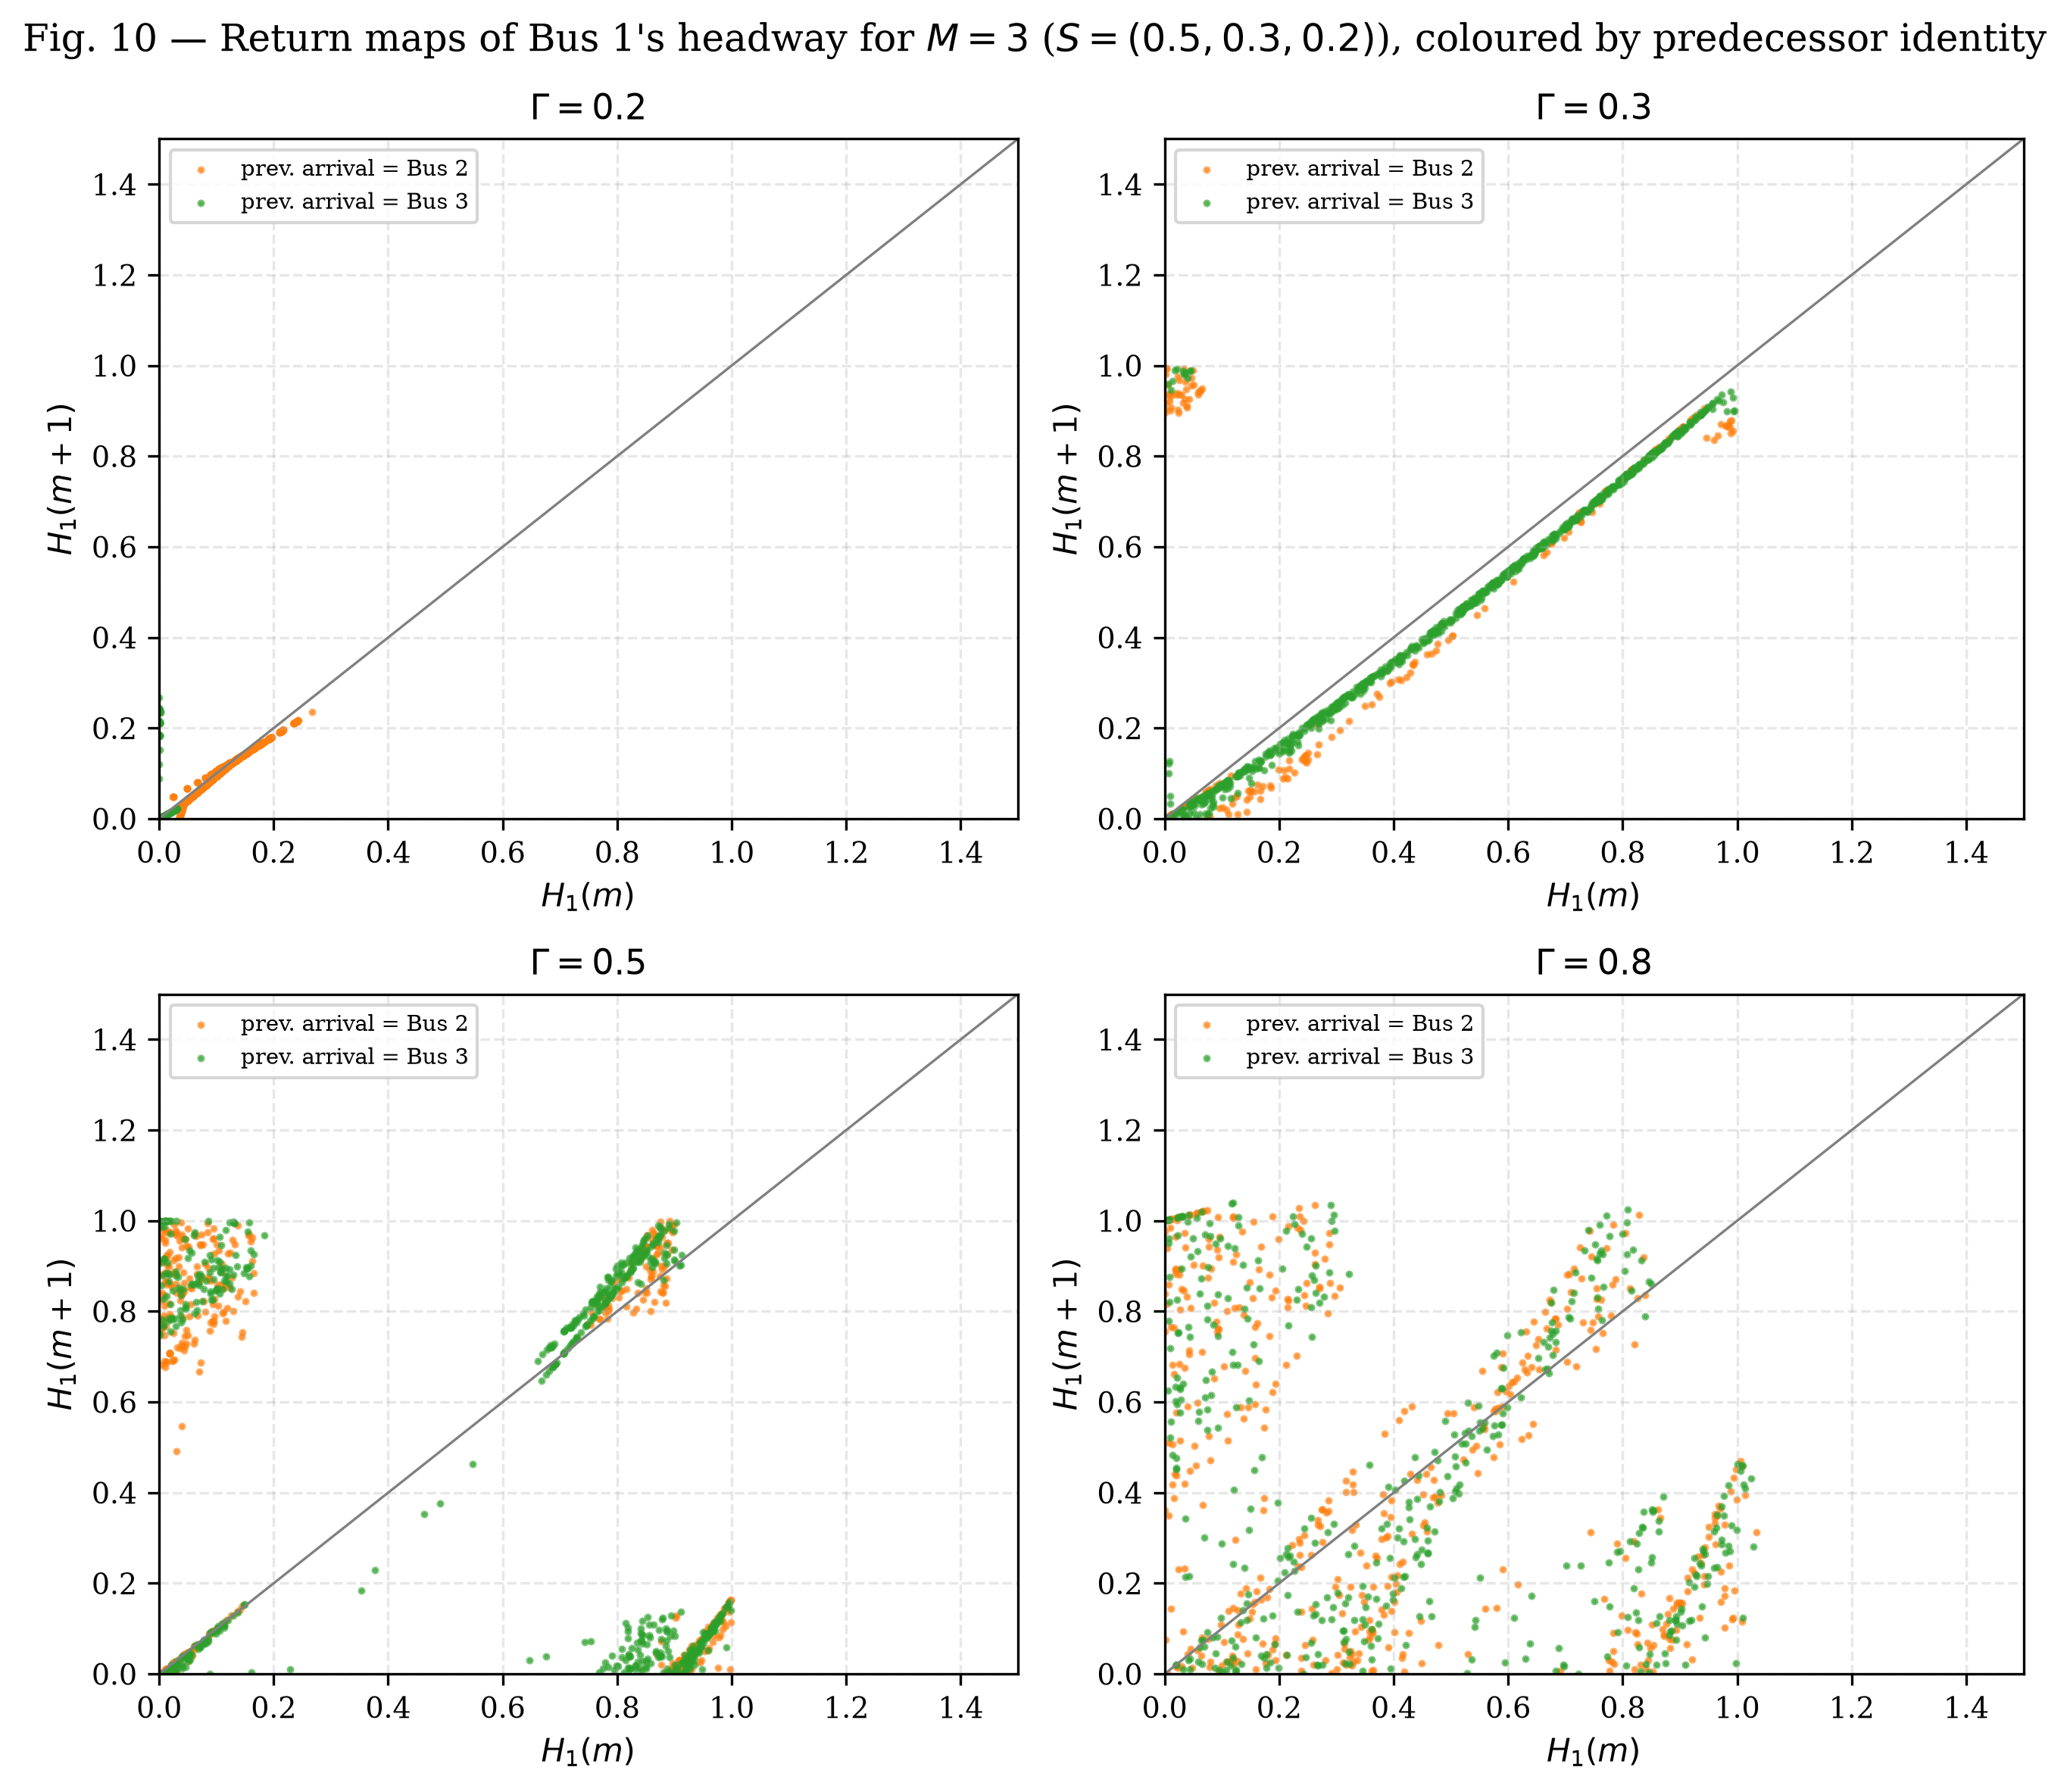
\includegraphics[width=0.85\textwidth,height=0.42\textheight,keepaspectratio]{fig10_three_bus_returnmap.png}
    \caption{$M=3$ return maps for Bus~1, coloured by predecessor identity. At high $\Gamma$ the two branches separate: the same $H_1(m)$ maps to different $H_1(m+1)$ depending on which bus preceded it.}
    \label{fig:fig10_three_bus}
\end{figure*}

With $M=2$ each bus has one possible predecessor, so $H_1(m+1)=f(H_1(m))$ is a true function. With $M=3$, Bus~1's predecessor alternates between Buses~2 and~3. Figure~\ref{fig:fig10_three_bus} colours points by predecessor. At $\Gamma=0.2$--$0.3$ the branches nearly overlap; by $\Gamma=0.5$--$0.8$ they visibly separate. The map $H_1(m+1)=f(H_1(m))$ is therefore \emph{not a function} of a single variable---the attractor lives in a genuinely higher-dimensional state space, though the dynamics remain completely deterministic once predecessor identity is included.

\subsection{Phase Boundary and Speedup Ceiling (Fig.~11)}

\begin{figure*}[tbp]
    \centering
    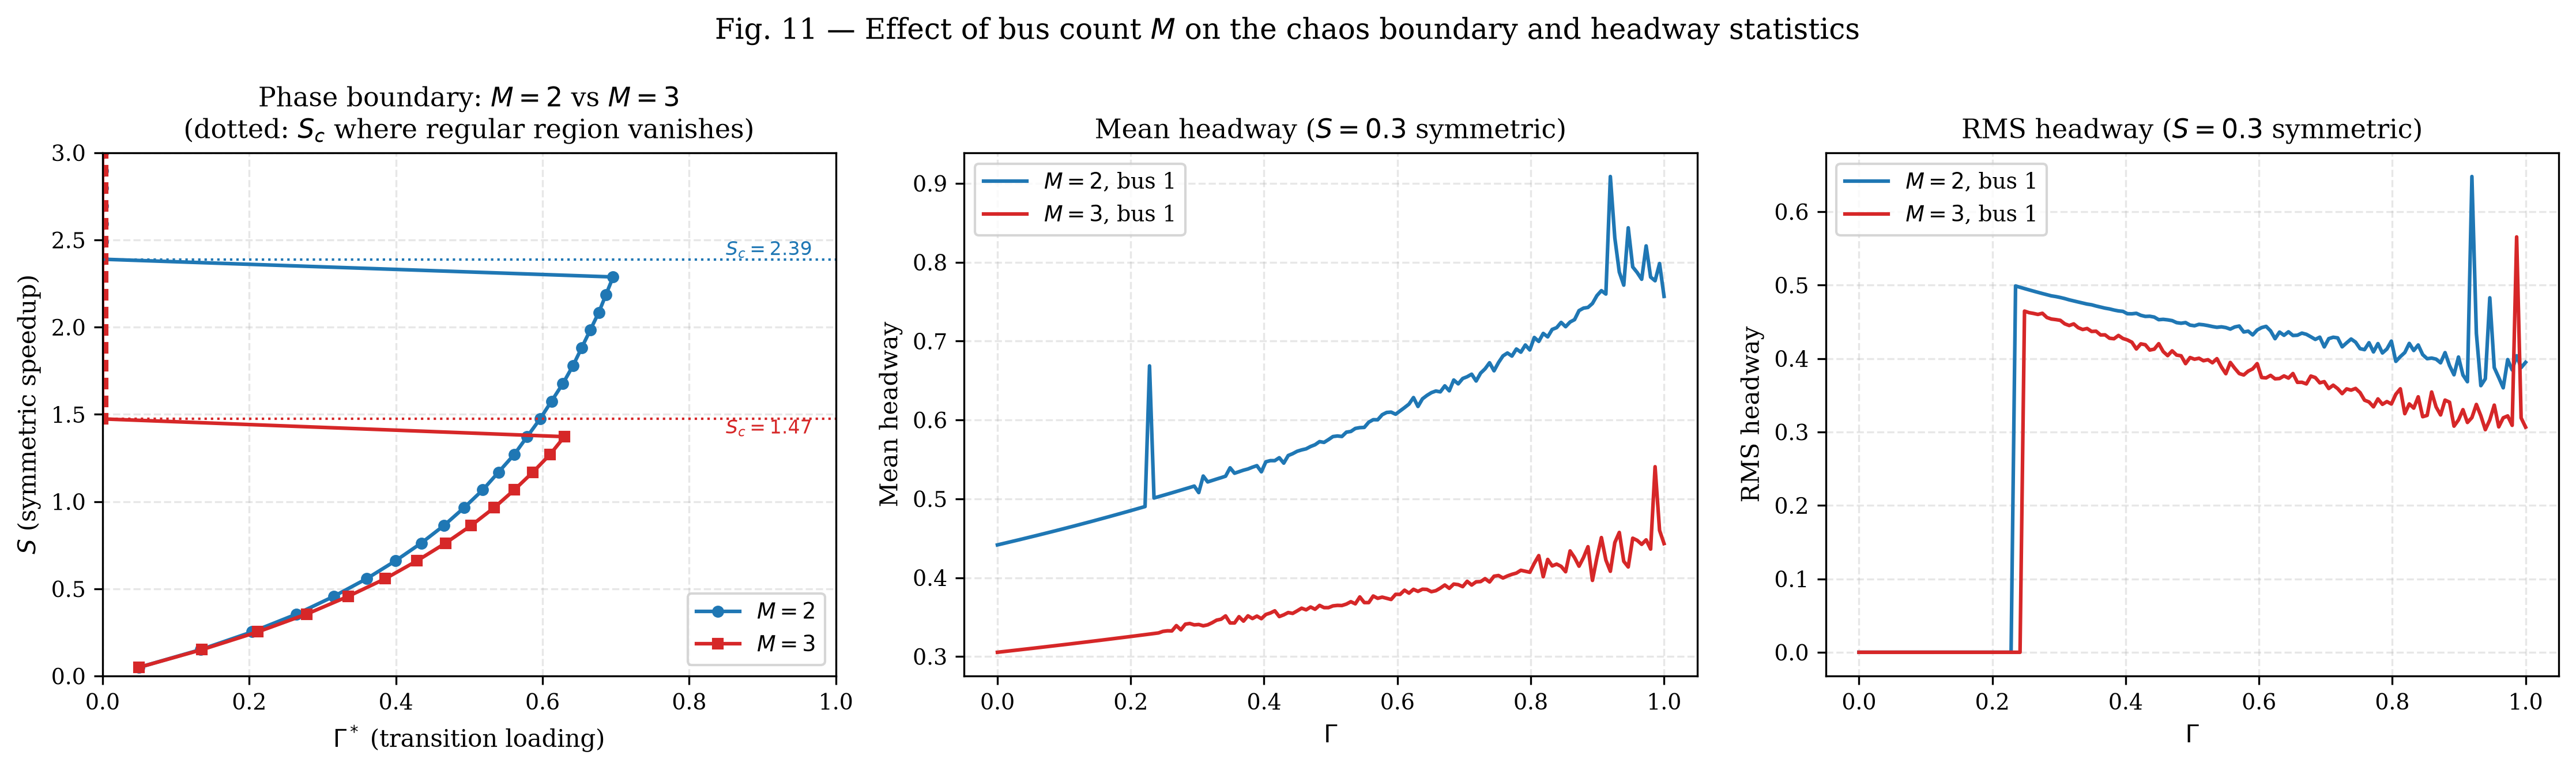
\includegraphics[width=\textwidth,height=0.30\textheight,keepaspectratio]{fig11_three_bus_phase.png}
    \caption{Left: phase boundary $\Gamma^*(S)$ for $M=2$ vs.\ $M=3$ (symmetric speedup); dotted lines mark $S_c$. Centre/right: mean and RMS headway at $S=0.3$.}
    \label{fig:fig11_three_bus}
\end{figure*}

Figure~\ref{fig:fig11_three_bus} compares $M=2$ and $M=3$ directly. Three findings:
\begin{enumerate}[leftmargin=*,itemsep=0pt,topsep=2pt]
    \item \textbf{$\Gamma^*$ barely changes with $M$.} For $S=0.25$: $\Gamma^*(M=2)=0.204$ vs.\ $\Gamma^*(M=3)=0.212$. The onset of chaos depends on the local feedback between consecutive arrivals, not on how many buses share the route.
    \item \textbf{Mean headway tightens.} At $\Gamma=0.3$, $S=0.3$: Bus~1's mean headway is $0.508$ with $M=2$ but only $0.341$ with $M=3$, close to the $2/3$ naive scaling, confirming the simulator correctly captures denser packing.
    \item \textbf{Speedup has a hard ceiling, lower for $M=3$.} Bisecting on $S$ at $\Gamma=0$ finds $S_c\approx2.0$ for $M=2$ and $S_c\approx1.6$ for $M=3$. Beyond $S_c$, the correction overcompensates every trip and generates chaos with no passenger load required. This is a mathematical property of the map when $\Gamma$ and $S$ are varied independently; physically, $\Gamma=\mu(\gamma+\eta)$ and $S_i\propto\mu(\gamma+\eta)$ share the same boarding-rate factor, so $\Gamma=0$ would also force $S_i=0$.
\end{enumerate}

\subsection{Summary: $M=3$ Generalises $M=2$}

The same map, the same algorithm, and the same diagnostic tools apply to $M=3$ without modification. Every qualitative insight---period-adding route to chaos, deterministic return-map structure, RMS-detectable transition, speedup as a bounded control---reproduces for three buses. Two new \emph{effects} (not mechanisms) emerge only at $M\geq3$: the return map becomes multi-valued in a single headway variable, and $S_c$ drops substantially. The formula and insights generalise; only numbers shift.

% ─────────────────────────────────────────────────────────────────────────────
\section{Interactive Demo}

A standalone browser demo (\texttt{sim.html}, no build step required) implements the same event-driven algorithm in JavaScript, animating buses around an elliptical track with arc-length-parameterised motion and plotting live per-bus return maps. Parameters $M\in[2,8]$, $\Gamma$, $S_i$, total trips and plot window are all adjustable. A screenshot is shown in Figure~\ref{fig:demo}.

\begin{figure}[htbp]
    \centering
    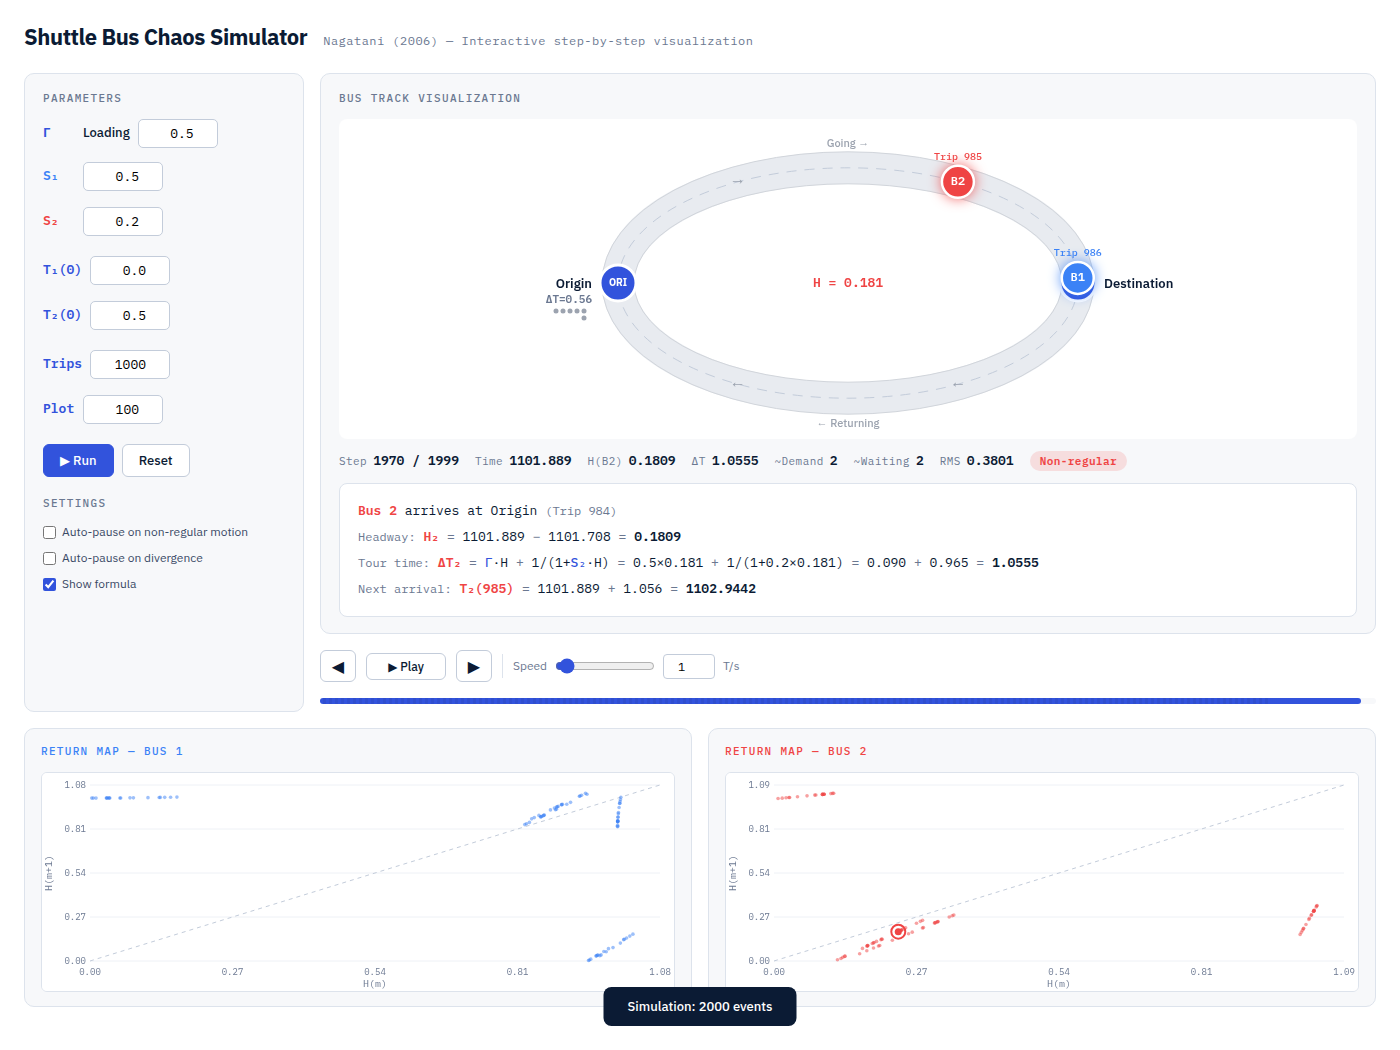
\includegraphics[width=\columnwidth,height=0.22\textheight,keepaspectratio]{demo_screenshot.png}
    \caption{Browser demo: animated track, formula breakdown, and live return maps.}
    \label{fig:demo}
\end{figure}

% ─────────────────────────────────────────────────────────────────────────────
\section{Conclusion}

We reproduced all figures of Nagatani~\cite{nagatani} for $M=2$ shuttle buses: period-adding bifurcations, piecewise-linear return maps confirming deterministic chaos, and a numerically determined phase boundary $\Gamma^*(S)$ showing speedup suppresses chaos with diminishing returns. Sensitivity tests show the attractor is unique (initial-condition independent) and structurally robust to timing noise up to 5\%, though fine periodic windows erode first. Extending to $M=3$ requires no new model; all qualitative findings generalise, with the return map becoming genuinely two-valued and the critical speedup ceiling dropping from $S_c\approx2.0$ to $\approx1.6$.

\printbibliography[heading=bibintoc,title={References}]

\end{document}
